\documentclass[aspectratio=43,9pt]{beamer}

\usepackage{iftex}
\ifPDFTeX
  \usepackage[T1]{fontenc}
  \usepackage[utf8]{inputenc}
  \usepackage[scaled=0.95]{helvet}
  \renewcommand{\familydefault}{\sfdefault}
\else
  \usepackage{fontspec}
  \setmainfont{TeX Gyre Heros}
  \setsansfont{TeX Gyre Heros}
  \setmonofont{Latin Modern Mono}
\fi

\usepackage{amsmath,amssymb,booktabs,tabularx,array,multirow}
\usepackage{listings}
\usepackage{xcolor}
\colorlet{blue}{black}
\colorlet{green}{black}
\colorlet{red}{black}
\colorlet{orange}{black}
\colorlet{magenta}{black}
\colorlet{teal}{black}
\colorlet{purple}{black}
\colorlet{cyan}{black}
\colorlet{pink}{black}
\usepackage{graphicx}
\usepackage{ragged2e}

\usetheme{default}
\setbeamertemplate{navigation symbols}{}
\setbeamertemplate{footline}[frame number]
\setbeamersize{text margin left=0.35cm,text margin right=0.35cm}
\setbeamercolor{frametitle}{fg=black,bg=white}
\setbeamerfont{frametitle}{series=\bfseries,size*={19}{21}}
\setbeamercolor{title}{fg=black}
\setbeamerfont{title}{series=\bfseries,size*={25}{27}}
\setbeamercolor{block title}{bg=black,fg=white}
\setbeamercolor{block body}{bg=white,fg=black}
\setbeamercolor{block title alerted}{bg=black,fg=white}
\setbeamercolor{block body alerted}{bg=white,fg=black}
\setbeamercolor{block title example}{bg=black,fg=white}
\setbeamercolor{block body example}{bg=white,fg=black}
\setbeamercolor{structure}{fg=black}
\setbeamercolor{itemize item}{fg=black}
\setbeamercolor{itemize subitem}{fg=black}
\setbeamerfont{block title}{series=\bfseries}
\setbeamertemplate{itemize item}{\color{black}\large\textbullet}
\setbeamertemplate{itemize subitem}{\color{black}\small\textbullet}
\setbeamertemplate{itemize subsubitem}{\color{black}\tiny\textbullet}
\setlength{\tabcolsep}{3pt}
\renewcommand{\arraystretch}{1.08}
\hypersetup{colorlinks=true,allcolors=black,urlcolor=black,linkcolor=black,citecolor=black}

\lstset{
  basicstyle=\ttfamily\tiny,
  breaklines=true,
  columns=fullflexible,
  keepspaces=true,
  showstringspaces=false,
  frame=single,
  framerule=0.2pt,
  xleftmargin=0pt,
  xrightmargin=0pt,
  aboveskip=2pt,
  belowskip=2pt
}

\newcommand{\graphplaceholder}[3][\linewidth]{%
  \fbox{\begin{minipage}[c][#2][c]{#1}\centering\scriptsize #3\end{minipage}}%
}

\newcommand{\reflink}[2]{\href{#1}{\mbox{#2}}}
\newcommand{\refline}[1]{%
  \par\vspace*{\fill}\hrule\vspace{0.2ex}{\fontsize{4.2}{4.5}\selectfont\raggedright\textbf{References: }#1\par}%
}

\begin{document}
% 1
\begin{frame}[plain]
\centering
\vspace{4.35em}
{\fontsize{25}{27}\selectfont\bfseries Evaluating Large Language\\[0.25em]Models Trained on Code (Codex)\par}
\vspace{2.1em}
{\tiny
M. Chen, J. Tworek, H. Jun, Q. Yuan, H. Ponde de Oliveira Pinto, J. Kaplan, H. Edwards, Y. Burda, N. Joseph, G. Brockman, A. Ray, R. Puri, G. Krueger, M. Petrov, H. Khlaaf, G. Sastry, P. Mishkin, B. Chan, S. Gray, N. Ryder, M. Pavlov, A. Power, L. Kaiser, M. Bavarian, C. Winter, P. Tillet, F. Petroski Such, D. Cummings, M. Plappert, F. Chantzis, E. Barnes, A. Herbert-Voss, W. Hebgen Guss, A. Nichol, A. Paino, N. Tezak, J. Tang, I. Babuschkin, S. Balaji, S. Jain, W. Saunders, C. Hesse, A. N. Carr, J. Leike, J. Achiam, V. Misra, E. Morikawa, A. Radford, M. Knight, M. Brundage, M. Murati, K. Mayer, P. Welinder, B. McGrew, D. Amodei, S. McCandlish, I. Sutskever, W. Zaremba\\[0.3em]
\reflink{https://arxiv.org/abs/2107.03374}{arXiv (2021)}}
\vfill
\end{frame}

% 4
\begin{frame}{A language model for code}
\small
\begin{block}{Program synthesis with language models}
\begin{itemize}
  \item Program synthesis is a longstanding challenge (Simon, 1963; Manna et al., 1971).
  \item Large code corpora became available, e.g. \textbf{CodeSearchNet} and \textbf{The Pile}.
  \item Self-supervised objectives used in NLP were adapted to code: \textbf{CodeBERT}, \textbf{T5}, and \textbf{PyMT5} are representative examples.
  \item Early analysis suggested that \textbf{GPT-3} could generate programs from Python docstrings even without explicit code-specialized training.
  \item Hypothesis of the paper: specializing a GPT language model for code could work across many tasks.
\end{itemize}
\end{block}

\begin{exampleblock}{This work: Codex}
Codex is a GPT-style model specialized for code. The paper positions it as a model that can generate useful code across tasks and notes that it is used for \textbf{Copilot}.
\end{exampleblock}

\refline{\href{https://arxiv.org/abs/2107.03374}{M. Chen et al., ``Evaluating Large Language Models Trained on Code, arXiv (2021)}; \href{https://arxiv.org/abs/1909.09436}{H. Husain et al., ``CodeSearchNet Challenge: Evaluating the State of Semantic Code Search, arXiv (2019)}; \href{https://arxiv.org/abs/2101.00027}{L. Gao et al., ``The Pile: An 800GB Dataset of Diverse Text for Language Modeling, arXiv (2020)}; \href{https://aclanthology.org/2020.findings-emnlp.139/}{Z. Feng et al., ``CodeBERT: A Pre-Trained Model for Programming and Natural Languages, Findings of EMNLP (2020)}; \href{https://proceedings.neurips.cc/paper/2020/hash/1457c0d6bfcb4967418bfb8ac142f64a-Abstract.html}{T. Brown et al., ``Language Models Are Few-Shot Learners, NeurIPS (2020)}; \href{https://www.eleuther.ai/projects/gpt-j/}{B. Wang and A. Komatsuzaki, ``GPT-J-6B: A 6 Billion Parameter Autoregressive Language Model, (2021)}.}
\end{frame}

% 52
\begin{frame}{Related Work}
\tiny
\begin{columns}[T,totalwidth=\textwidth]
\column{0.49\textwidth}
\begin{block}{Learning to Execute}
LSTMs are trained on programs and can learn algorithmic tasks such as adding two 9-digit numbers with about 99\% accuracy. Curriculum learning plays a key role.
\end{block}

\begin{block}{SPoC}
The SPoC dataset contains about 18K C++ programs and studies pseudocode-to-code synthesis using a seq2seq model with best-first search.
\end{block}

\column{0.49\textwidth}
\begin{block}{Naturalness of Software}
This work studies code with n-gram language models and shows that source code is statistically natural in ways that can be exploited for modeling and tooling.
\end{block}

\begin{block}{APPS}
APPS introduces a benchmark with 10K programming problems across three difficulty levels and includes test cases for evaluating generated solutions.
\end{block}
\end{columns}

\refline{\href{https://arxiv.org/abs/1410.4615}{W. Zaremba and I. Sutskever, ``Learning to Execute, arXiv (2014)}; \href{https://dl.acm.org/doi/10.1109/ICSE.2012.6227135}{A. Hindle et al., ``On the Naturalness of Software, ICSE (2012)}; \href{https://proceedings.neurips.cc/paper/2019/hash/7298332f04ac004a0ca44cc69ecf6f6b-Abstract.html}{S. Kulal et al., ``SPoC: Search-Based Pseudocode to Code, NeurIPS (2019)}; \href{https://proceedings.neurips.cc/paper/2021/hash/c24cd76e1ce41366a4bbe8a49b02a028-Abstract.html}{D. Hendrycks et al., ``Measuring Coding Challenge Competence With APPS, NeurIPS (2021)}.}
\end{frame}

% importance
\begin{frame}{Importance: why this paper changed the field}
\scriptsize
\begin{columns}[T,totalwidth=\textwidth]
\column{0.32\textwidth}
\begin{block}{Before Codex}
\begin{itemize}
  \item Program synthesis and code modeling already existed, but results were often shown on constrained tasks or with weaker text-similarity metrics.
  \item The field still lacked a simple execution-based story for answering: can a language model actually solve a programming task?
\end{itemize}
\end{block}

\column{0.34\textwidth}
\begin{block}{What Codex changed}
\begin{itemize}
  \item It combined a large code-specialized LM with a clean hand-written benchmark.
  \item It made \textbf{functional correctness} and \textbf{pass@k} the central evaluation language for code generation.
  \item It shifted the question from ``can LMs autocomplete code?'' to ``how often can they solve a task?''
\end{itemize}
\end{block}

\column{0.32\textwidth}
\begin{exampleblock}{After Codex}
\begin{itemize}
  \item The area moved toward stronger coding assistants, open code LMs, and harder benchmarks.
  \item Follow-up work pushed on competition-level generation, open model releases, and repository-level software engineering evaluation.
\end{itemize}
\end{exampleblock}
\end{columns}

\refline{\href{https://arxiv.org/abs/2107.03374}{M. Chen et al., ``Evaluating Large Language Models Trained on Code,'' arXiv (2021)}; \href{https://arxiv.org/abs/2203.07814}{Y. Li et al., ``Competition-Level Code Generation with AlphaCode,'' Science (2022)}; \href{https://arxiv.org/abs/2305.06161}{L. Ben Allal et al., ``StarCoder: May the Source Be with You!,'' arXiv (2023)}; \href{https://arxiv.org/abs/2308.12950}{B. Roziere et al., ``Code Llama: Open Foundation Models for Code,'' arXiv (2023)}; \href{https://arxiv.org/abs/2310.06770}{J. Jimenez et al., ``SWE-bench: Can Language Models Resolve Real-World GitHub Issues?,'' ICLR (2024)}.}
\end{frame}


% 5
\begin{frame}{Task and approach}
\scriptsize
\begin{columns}[T,totalwidth=\textwidth]
\column{0.49\textwidth}
\begin{block}{Task: functions from docstrings}
\begin{itemize}
  \item Input: \textbf{docstring}
  \item Output: \textbf{Python function}
  \item Code correctness is evaluated automatically via \textbf{unit tests}.
  \item This differs from natural language generation, which usually needs human assessors or heuristic metrics.
  \item For benchmarking, the paper constructs \textbf{164 original programming problems} with tests.
  \item Problem types include language comprehension, algorithms, simple mathematics, and interview-style questions.
\end{itemize}
\end{block}

\column{0.49\textwidth}
\begin{block}{Problem solving with one sample}
Approach: generate samples and check whether any pass the unit tests.
\begin{itemize}
  \item Codex (12B): \textbf{28.8\%}
  \item Codex (300M): \textbf{13.2\%}
  \item GPT-J (6B): \textbf{11.4\%}
  \item Other GPT models: approximately \textbf{0\%}
  \item After supervised fine-tuning on correct implementations, Codex-S (12B) reaches \textbf{37.7\%}
\end{itemize}
\end{block}

\begin{exampleblock}{Problem solving with multiple samples}
Programming usually involves iteration and bug fixing. Repeated sampling approximates this process.
\begin{itemize}
  \item Codex-S (12B) with 100 samples solves \textbf{77.5\%} of problems.
  \item Selecting the sample with highest mean log-probability solves \textbf{44.5\%}.
\end{itemize}
\end{exampleblock}
\end{columns}

\refline{\href{https://arxiv.org/abs/2107.03374}{M. Chen et al., ``Evaluating Large Language Models Trained on Code, arXiv (2021)}; \href{https://www.eleuther.ai/projects/gpt-j/}{B. Wang and A. Komatsuzaki, ``GPT-J-6B: A 6 Billion Parameter Autoregressive Language Model, (2021)}.}
\end{frame}

% 7
\begin{frame}{Evaluation framework}
\scriptsize
\begin{columns}[T,totalwidth=\textwidth]
\column{0.52\textwidth}
\begin{block}{Functional correctness}
\begin{itemize}
  \item Match-based metrics compare against a reference exactly or fuzzily (e.g. BLEU).
  \item Such metrics are limited for code because many different programs can be equivalent.
  \item The paper therefore emphasizes \textbf{functional correctness}: a sample is correct if it passes a set of unit tests.
  \item This is also how human developers judge code in practice, e.g. via test-driven development and CI.
\end{itemize}
\end{block}

\column{0.46\textwidth}
\begin{block}{The \texttt{pass@k} metric}
Generate \(k\) samples per problem. A problem is solved if \emph{any} sample passes the tests.

\vspace{0.4em}
Unbiased estimator used in the paper:
\[
\mathrm{pass@}k \;\triangleq\; \mathbb{E}_{\text{problems}}\!\left[1 - \frac{\binom{n-c}{k}}{\binom{n}{k}}\right]
\]
where \(n \ge k\) is the number of samples and \(c\) is the number of correct samples among them.

Advantage: using more generated samples reduces variance while keeping comparisons fair.
\end{block}
\end{columns}

\refline{\href{https://arxiv.org/abs/2107.03374}{M. Chen et al., ``Evaluating Large Language Models Trained on Code, arXiv (2021)}; \href{https://aclanthology.org/P02-1040/}{K. Papineni et al., ``BLEU: A Method for Automatic Evaluation of Machine Translation, ACL (2002)}; \href{https://arxiv.org/abs/2009.10297}{S. Ren et al., ``CodeBLEU: A Method for Automatic Evaluation of Code Synthesis, arXiv (2020)}; \href{https://proceedings.neurips.cc/paper/2020/hash/ed23fbf18c2cd35f8c7f8de44f85c08d-Abstract.html}{B. Roziere et al., ``Unsupervised Translation of Programming Languages, NeurIPS (2020)}; \href{https://proceedings.neurips.cc/paper/2019/hash/7298332f04ac004a0ca44cc69ecf6f6b-Abstract.html}{S. Kulal et al., ``SPoC: Search-Based Pseudocode to Code, NeurIPS (2019)}.}
\end{frame}

% 11
\begin{frame}{Evaluation details}
\scriptsize
\begin{block}{HumanEval: hand-written evaluation set}
\begin{itemize}
  \item Functional correctness is evaluated on \textbf{164 hand-written problems}.
  \item Each HumanEval problem contains a function signature, a docstring, a body, and several unit tests (average: \textbf{7.7} tests per problem).
  \item Hand-written problems matter because the models are trained on GitHub, where many public benchmark solutions already exist.
  \item HumanEval targets simple mathematics, reasoning, and language comprehension.
  \item The dataset is made public for future benchmarking.
\end{itemize}
\end{block}

\begin{block}{Sandbox for executing generated programs}
\begin{itemize}
  \item Executing public code and generated code creates a security risk.
  \item The paper therefore runs untrusted programs in a sandboxed environment.
  \item \textbf{\reflink{https://gvisor.dev/}{gVisor}} is used to isolate the host, and network-adjacent services are protected with eBPF-based firewall rules.
\end{itemize}
\end{block}

\refline{\href{https://arxiv.org/abs/2107.03374}{M. Chen et al., ``Evaluating Large Language Models Trained on Code, arXiv (2021)}; \href{https://proceedings.neurips.cc/paper/2021/hash/c24cd76e1ce41366a4bbe8a49b02a028-Abstract.html}{D. Hendrycks et al., ``Measuring Coding Challenge Competence With APPS, NeurIPS (2021)}; \href{https://github.com/openai/human-eval}{OpenAI, ``HumanEval benchmark repository}; \href{https://gvisor.dev/}{Google, ``gVisor sandboxed container runtime}.}
\end{frame}


% 13
\begin{frame}{Code Fine-tuning}
\scriptsize
\begin{block}{Overview}
Codex is produced by fine-tuning GPT models of up to \textbf{12B} parameters. Unlike GPT models trained only on text, Codex obtains non-trivial HumanEval performance, and with 100 samples per problem, the majority of problems have at least one solution.
\end{block}

\begin{columns}[T,totalwidth=\textwidth]
\column{0.50\textwidth}
\begin{block}{Data collection and fine-tuning}
\begin{itemize}
  \item Training corpus collected in May 2020 from \textbf{54M GitHub repositories}.
  \item Produced \textbf{179 GB} of unique Python files under 1 MB.
  \item Filtering removed likely auto-generated files, very long lines, and files with a very small fraction of alphanumerics.
  \item Final result: \textbf{159 GB} of unique Python files.
  \item Surprisingly, fine-tuning from GPT-3 gave no improvement over training from scratch, although it converged faster and was used in practice.
\end{itemize}
\end{block}

\column{0.47\textwidth}
\begin{block}{Optimization and tokenization}
\begin{itemize}
  \item Same learning rate as the corresponding GPT model.
  \item Linear warmup for 175 steps; cosine decay afterwards.
  \item Training on \textbf{100B tokens} with Adam \((\beta_1=0.9,\,\beta_2=0.95,\,\epsilon=10^{-8})\) and weight decay 0.1.
  \item GPT-3 tokenization is reused, but extra whitespace tokens are added for code.
  \item This reduces the token count for code by roughly \textbf{30\%}.
\end{itemize}
\end{block}
\end{columns}

\refline{\href{https://arxiv.org/abs/2107.03374}{M. Chen et al., ``Evaluating Large Language Models Trained on Code, arXiv (2021)}; \href{https://arxiv.org/abs/1412.6980}{D. P. Kingma and J. Ba, ``Adam: A Method for Stochastic Optimization, ICLR (2015)}.}
\end{frame}

% 24
\begin{frame}{Supervised Fine-tuning}
\scriptsize
\begin{block}{Overview}
GitHub data contains far more than clean ``function from docstring'' examples: it also includes classes, config files, scripts, and data files. This mismatch may limit HumanEval performance, so the paper builds a supervised training set of standalone function-completion tasks.
\end{block}

\begin{block}{Source 1: competitive programming problems}
\begin{itemize}
  \item Problems, solutions, and function signatures were collected from interview-preparation and programming-contest websites.
  \item Problem descriptions are used as docstrings.
  \item Unit tests are created from examples in statements and by submitting incorrect solutions to reveal hidden cases.
  \item These sources provide self-contained tasks with strong algorithmic content and usually good test coverage.
  \item Roughly \textbf{10,000} problems are curated from these sources.
\end{itemize}
\end{block}

\refline{\href{https://arxiv.org/abs/2107.03374}{M. Chen et al., ``Evaluating Large Language Models Trained on Code, arXiv (2021)}.}
\end{frame}

% 25
\begin{frame}{Supervised Fine-tuning}
\scriptsize
\begin{block}{Source 2: problems from Continuous Integration}
\begin{itemize}
  \item Problems are also extracted from open-source repositories by tracing inputs and outputs during integration tests with \texttt{sys.setprofile}.
  \item CI config files reveal how to create environments, install dependencies, and run tests.
  \item Repositories using \textbf{Travis} or \textbf{\reflink{https://tox.wiki/}{Tox}} are particularly useful; additional source is pulled from PyPI.
  \item Because the code is untrusted, all integration tests are executed in the sandbox.
  \item Only about \textbf{40,000} problems are collected from millions of functions, mainly because not all functions are easy to trace and some runtime objects cannot be restored outside the sandbox.
\end{itemize}
\end{block}

\begin{block}{Filtering problems}
\begin{itemize}
  \item Automatically gathered prompts may be ambiguous or stateful.
  \item Codex-12B is used to generate 100 samples per problem.
  \item If all samples fail, the problem is discarded as too hard or ambiguous.
  \item Verification is rerun multiple times to filter out stateful problems.
\end{itemize}
\end{block}

\refline{\href{https://arxiv.org/abs/2107.03374}{M. Chen et al., ``Evaluating Large Language Models Trained on Code, arXiv (2021)}; \href{https://www.travis-ci.com/}{Travis CI documentation}; \href{https://tox.wiki/}{Tox documentation}.}
\end{frame}

% 26
\begin{frame}[fragile]{Supervised Fine-tuning}
\scriptsize
\begin{columns}[T,totalwidth=\textwidth]
\column{0.52\textwidth}
\begin{block}{Methodology - training with prompts}
Training examples are assembled in the same prompt format used at evaluation time.
\begin{lstlisting}
def solution(lst):
    """Given a non-empty list of integers, return the sum
    of all odd elements that are in even positions.

    Examples
    solution([5, 8, 7, 1]) => 12
    solution([3, 3, 3, 3, 3]) => 9
    solution([30, 13, 24, 321]) => 0
    """
    return sum(lst[i] for i in range(0, len(lst))
               if i % 2 == 0 and lst[i] % 2 == 1)
\end{lstlisting}
\begin{itemize}
  \item Codex is fine-tuned on these training problems to produce \textbf{Codex-S}.
  \item Training minimizes the negative log-likelihood of the reference solution while masking the prompt.
  \item Shorter prompts are left-padded so the target solutions line up.
  \item Learning rate is 1/10 of Codex with the same schedule until validation loss plateaus (after fewer than 10B tokens).
\end{itemize}
\end{block}

\column{0.44\textwidth}
\begin{block}{Optimal temperatures}
\begin{itemize}
  \item Codex-S prefers higher temperatures than Codex for all cases with \(k>1\).
  \item The paper suggests this may reflect a narrower learned distribution.
  \item For later evaluation:
    \begin{itemize}
      \item \(T^*=0\) for \texttt{pass@1}
      \item \(T^*=1\) for \texttt{pass@100}
    \end{itemize}
\end{itemize}
\end{block}

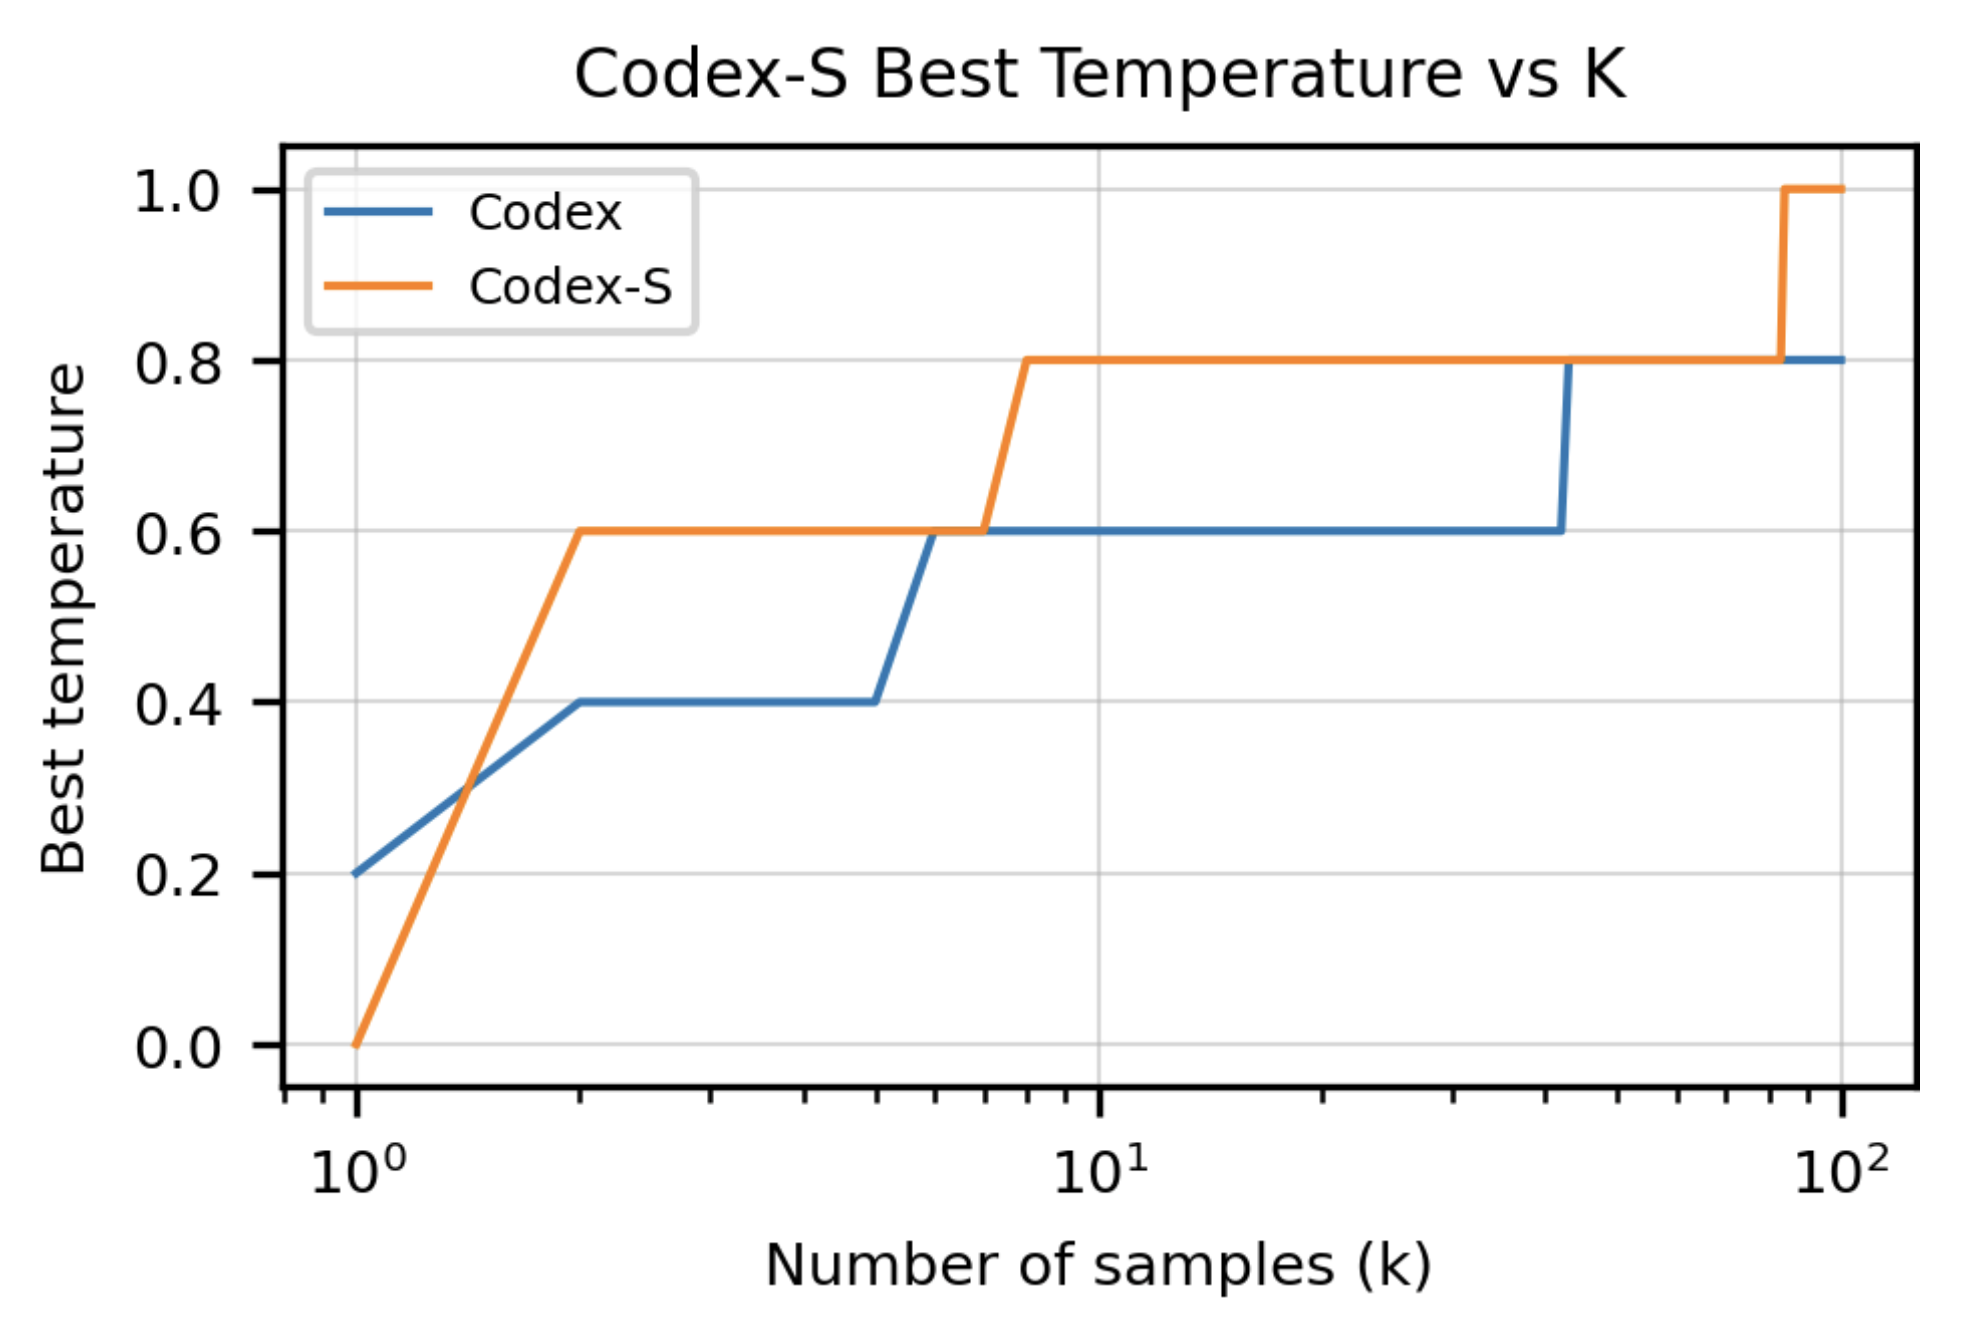
\includegraphics[width=0.9\textwidth]{temp.png}\end{columns}

\refline{\href{https://arxiv.org/abs/2107.03374}{M. Chen et al., ``Evaluating Large Language Models Trained on Code, arXiv (2021)}.}
\end{frame}

% 19
\begin{frame}{Comparative Analysis of Related Models}
\tiny
\begin{columns}[T,totalwidth=\textwidth]
\column{0.27\textwidth}
\begin{block}{Related approaches}
\begin{itemize}
  \item GPT-Neo and GPT-J-6B are the closest comparison points.
  \item Both are trained on The Pile, of which about 8\% comes from GitHub.
  \item GPT-J-6B already produces qualitatively reasonable code.
\end{itemize}
\end{block}

\begin{block}{Temperatures}
GPT-Neo: 0.2, 0.4, 0.8\\
GPT-J-6B: 0.2, 0.8\\
Tabnine: 0.4, 0.8
\end{block}

\column{0.49\textwidth}
\begin{block}{HumanEval results}
\begin{tabular}{lccc}
\toprule
Model & \(k=1\) & \(k=10\) & \(k=100\)\\
\midrule
GPT-Neo 125M & 0.75\% & 1.88\% & 2.97\%\\
GPT-Neo 1.3B & 4.79\% & 7.47\% & 16.30\%\\
GPT-Neo 2.7B & 6.41\% & 11.27\% & 21.37\%\\
GPT-J 6B & 11.62\% & 15.74\% & 27.74\%\\
Tabnine & 2.58\% & 4.35\% & 7.59\%\\
\midrule
Codex-12M & 2.00\% & 3.62\% & 8.58\%\\
Codex-25M & 3.21\% & 7.10\% & 12.89\%\\
Codex-42M & 5.06\% & 8.80\% & 15.55\%\\
Codex-85M & 8.22\% & 12.81\% & 22.40\%\\
Codex-300M & 13.17\% & 20.37\% & 36.27\%\\
Codex-679M & 16.22\% & 25.70\% & 40.95\%\\
Codex-2.5B & 21.36\% & 35.42\% & 59.50\%\\
Codex-12B & 28.81\% & 46.81\% & 72.31\%\\
\bottomrule
\end{tabular}
\end{block}

\column{0.22\textwidth}
\begin{alertblock}{Takeaway}
Codex-12B goes considerably beyond the performance of prior models.
\end{alertblock}

\begin{exampleblock}{Parameter note}
Codex-300M achieves this despite having roughly \textbf{20x fewer parameters than GPT-J-6B}. 
\end{exampleblock}
\end{columns}

\refline{\href{https://arxiv.org/abs/2107.03374}{M. Chen et al., ``Evaluating Large Language Models Trained on Code, arXiv (2021)}; \href{https://github.com/EleutherAI/gpt-neo}{S. Black et al., ``GPT-Neo: Large Scale Autoregressive Language Modeling with Mesh-Tensorflow, (2021)}; \href{https://www.eleuther.ai/projects/gpt-j/}{B. Wang and A. Komatsuzaki, ``GPT-J-6B: A 6 Billion Parameter Autoregressive Language Model, (2021)}; \href{https://arxiv.org/abs/2101.00027}{L. Gao et al., ``The Pile: An 800GB Dataset of Diverse Text for Language Modeling, arXiv (2020)}.}
\end{frame}

% 20
\begin{frame}{Results on the APPS Dataset}
\tiny
\begin{columns}[T,totalwidth=\textwidth]
\column{0.44\textwidth}
\begin{block}{APPS dataset comparison}
\begin{itemize}
  \item APPS was introduced to measure coding challenge competence.
  \item It contains \textbf{5000 train} and \textbf{5000 test} coding problems.
  \item Each example includes unit tests; training examples also include solutions.
  \item Most APPS tasks are \textbf{full-program synthesis} problems (stdin/stdout), not single-function generation.
  \item Original APPS metrics: \textbf{strict accuracy} and \textbf{test case average}.
  \item Codex results here are reported only under strict accuracy / \texttt{pass@k}.
\end{itemize}
\end{block}

\column{0.54\textwidth}
\begin{block}{Implementation details and results}
\begin{itemize}
  \item Example cases: APPS gives 3 I/O examples; Codex uses one example as a formatting hint (``1-shot'').
  \item Timeouts: results are reported both with and without counting solutions that pass tests but time out after 3 seconds.
\end{itemize}

\begin{tabular}{lccc}
\toprule
Method & Intro & Interview & Competition\\
\midrule
GPT-Neo 2.7B raw \texttt{p@1} & 3.90 & 0.57 & 0.00\\
GPT-Neo 2.7B raw \texttt{p@5} & 5.50 & 0.80 & 0.00\\
1-shot Codex raw \texttt{p@1} & 4.14 (4.33) & 0.14 (0.30) & 0.02 (0.03)\\
1-shot Codex raw \texttt{p@5} & 9.65 (10.05) & 0.51 (1.02) & 0.09 (0.16)\\
1-shot Codex raw \texttt{p@100} & 20.20 (21.57) & 2.04 (3.99) & 1.05 (1.73)\\
1-shot Codex raw \texttt{p@1000} & 25.02 (27.77) & 3.70 (7.94) & 2.33 (5.85)\\
1-shot Codex filtered \texttt{p@1} & 22.78 (25.10) & 2.64 (5.78) & 3.04 (5.25)\\
1-shot Codex filtered \texttt{p@5} & 24.52 (27.15) & 3.23 (7.13) & 3.08 (5.53)\\
\bottomrule
\end{tabular}

Temperature 0.6 is used for all \(k\) in \texttt{pass@k}.
\end{block}
\end{columns}

\refline{\href{https://arxiv.org/abs/2107.03374}{M. Chen et al., ``Evaluating Large Language Models Trained on Code, arXiv (2021)}; \href{https://proceedings.neurips.cc/paper/2021/hash/c24cd76e1ce41366a4bbe8a49b02a028-Abstract.html}{D. Hendrycks et al., ``Measuring Coding Challenge Competence With APPS, NeurIPS (2021)}; \href{https://github.com/EleutherAI/gpt-neo}{S. Black et al., ``GPT-Neo: Large Scale Autoregressive Language Modeling with Mesh-Tensorflow, (2021)}.}
\end{frame}

% 27
\begin{frame}{Supervised Fine-tuning: Results}
\scriptsize
\begin{columns}[T,totalwidth=\textwidth]
\column{0.49\textwidth}
\begin{block}{Influence of model size}
\begin{itemize}
  \item Codex-S beats Codex by an average of \textbf{6.5\%} on \texttt{pass@1}.
  \item On \texttt{pass@100}, the average gain is \textbf{15.1\%}.
\end{itemize}
\end{block}

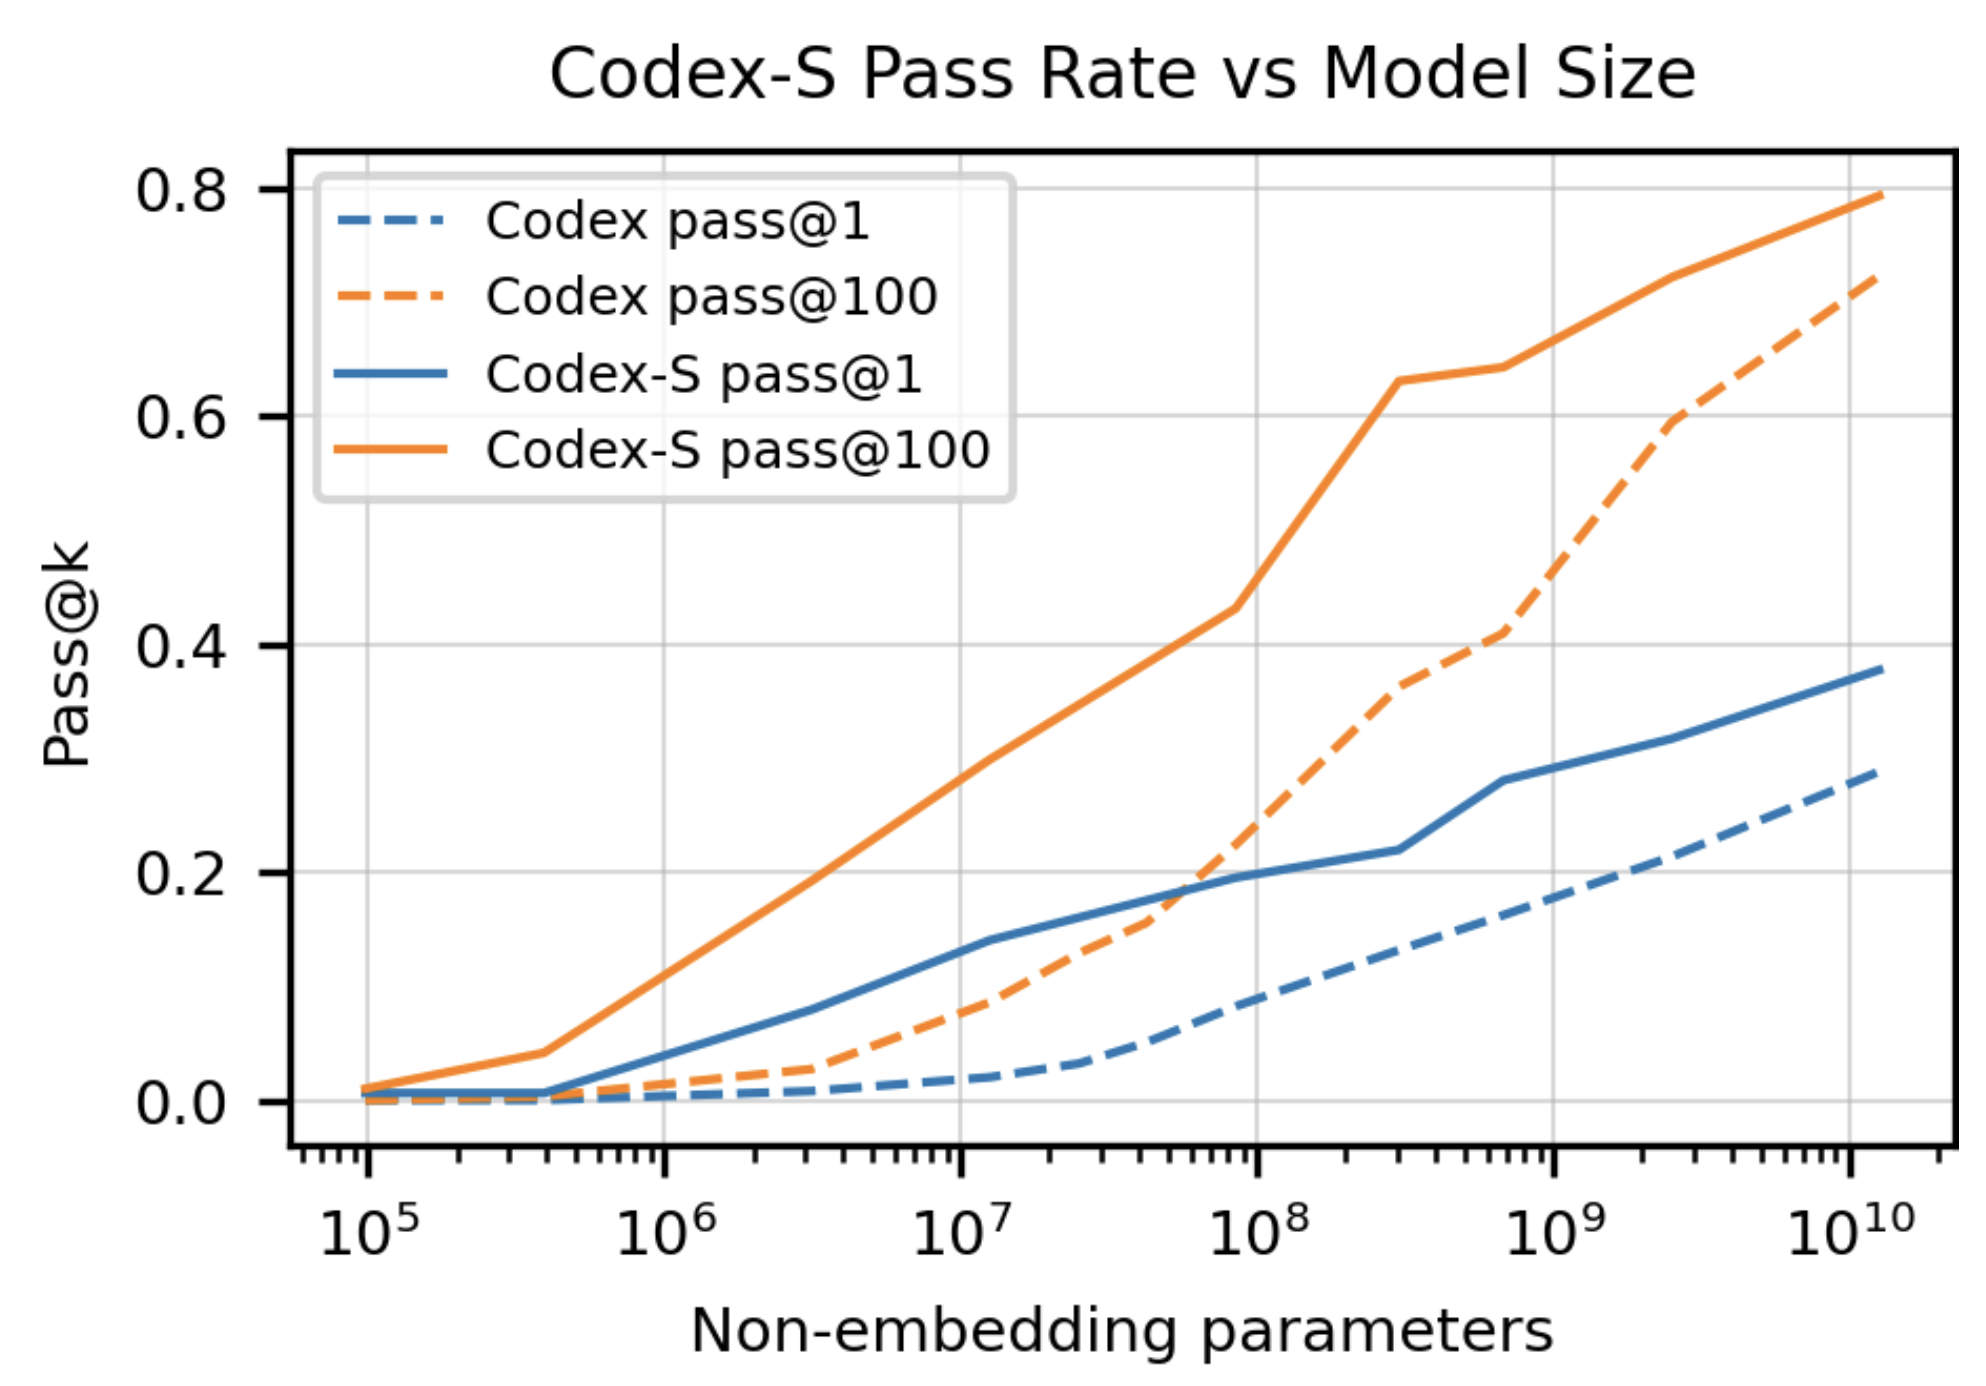
\includegraphics[width=0.9\textwidth]{s1.png}

\column{0.49\textwidth}
\begin{block}{Sample ranking heuristics}
\begin{itemize}
  \item Oracle reranking remains an upper bound.
  \item Mean log-probability is again the best practical heuristic.
  \item The average benefit of mean log-probability is about \textbf{2\% higher} for Codex-S than for Codex.
\end{itemize}
\end{block}

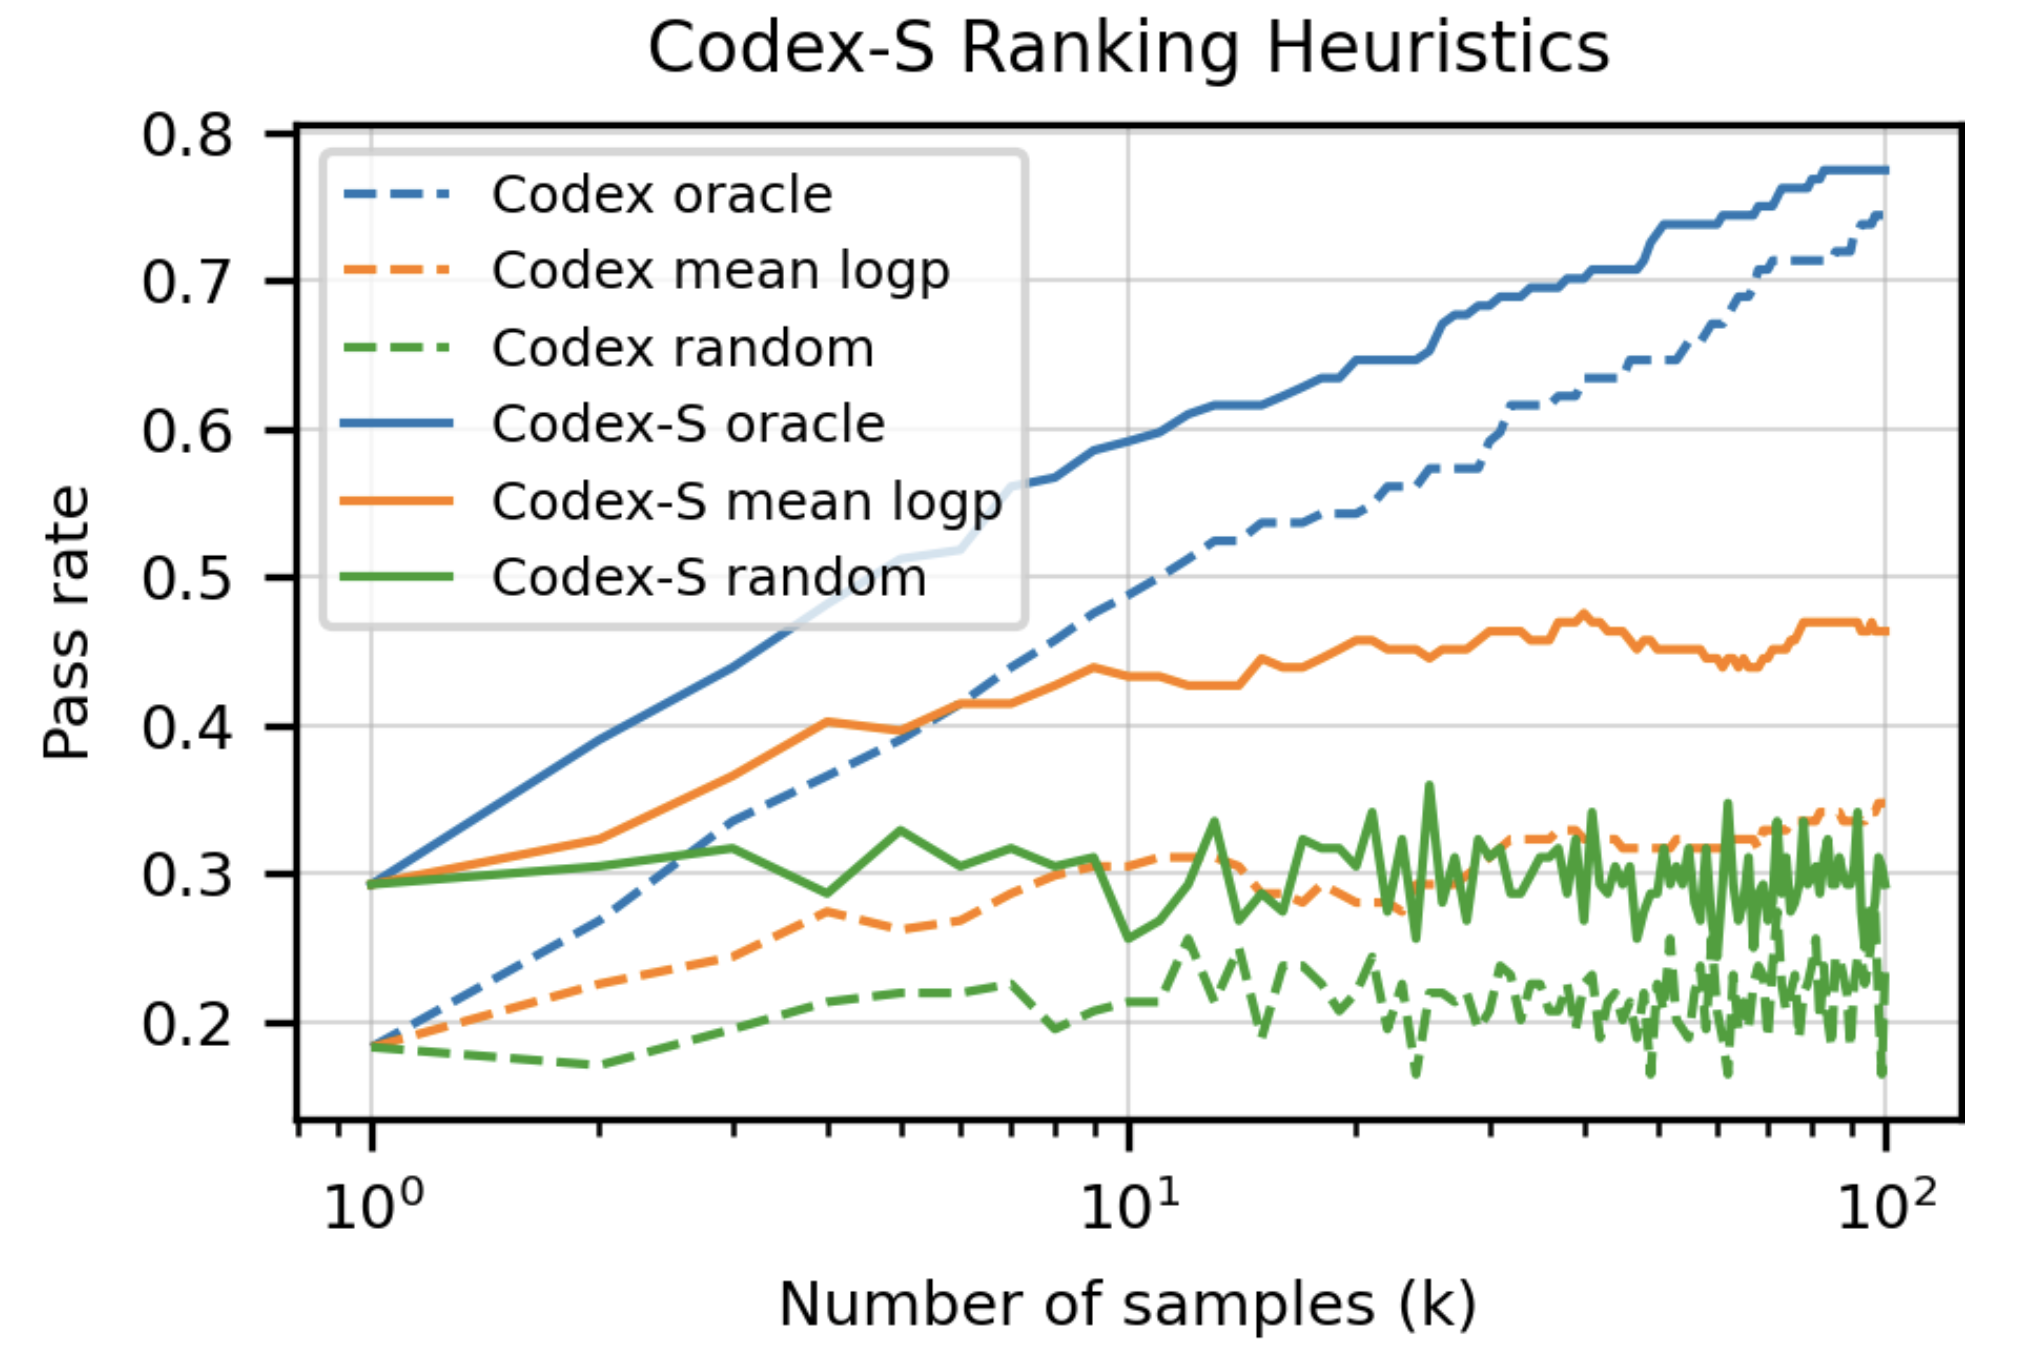
\includegraphics[width=0.9\textwidth]{s2.png}
\end{columns}

\refline{\href{https://arxiv.org/abs/2107.03374}{M. Chen et al., ``Evaluating Large Language Models Trained on Code, arXiv (2021)}.}
\end{frame}

% 28
\begin{frame}{Comparing Codex and Codex-S}
\small
\begin{block}{Comparing training strategies on HumanEval}
\begin{itemize}
  \item \textbf{Codex-S mean-logp reranking} solves \textbf{44.5\%} when reranking 100 samples.
  \item \textbf{Codex-S oracle reranking} solves \textbf{77.5\%} when selecting from 100 samples using the unit tests.
\end{itemize}
\end{block}
\begin{center}
    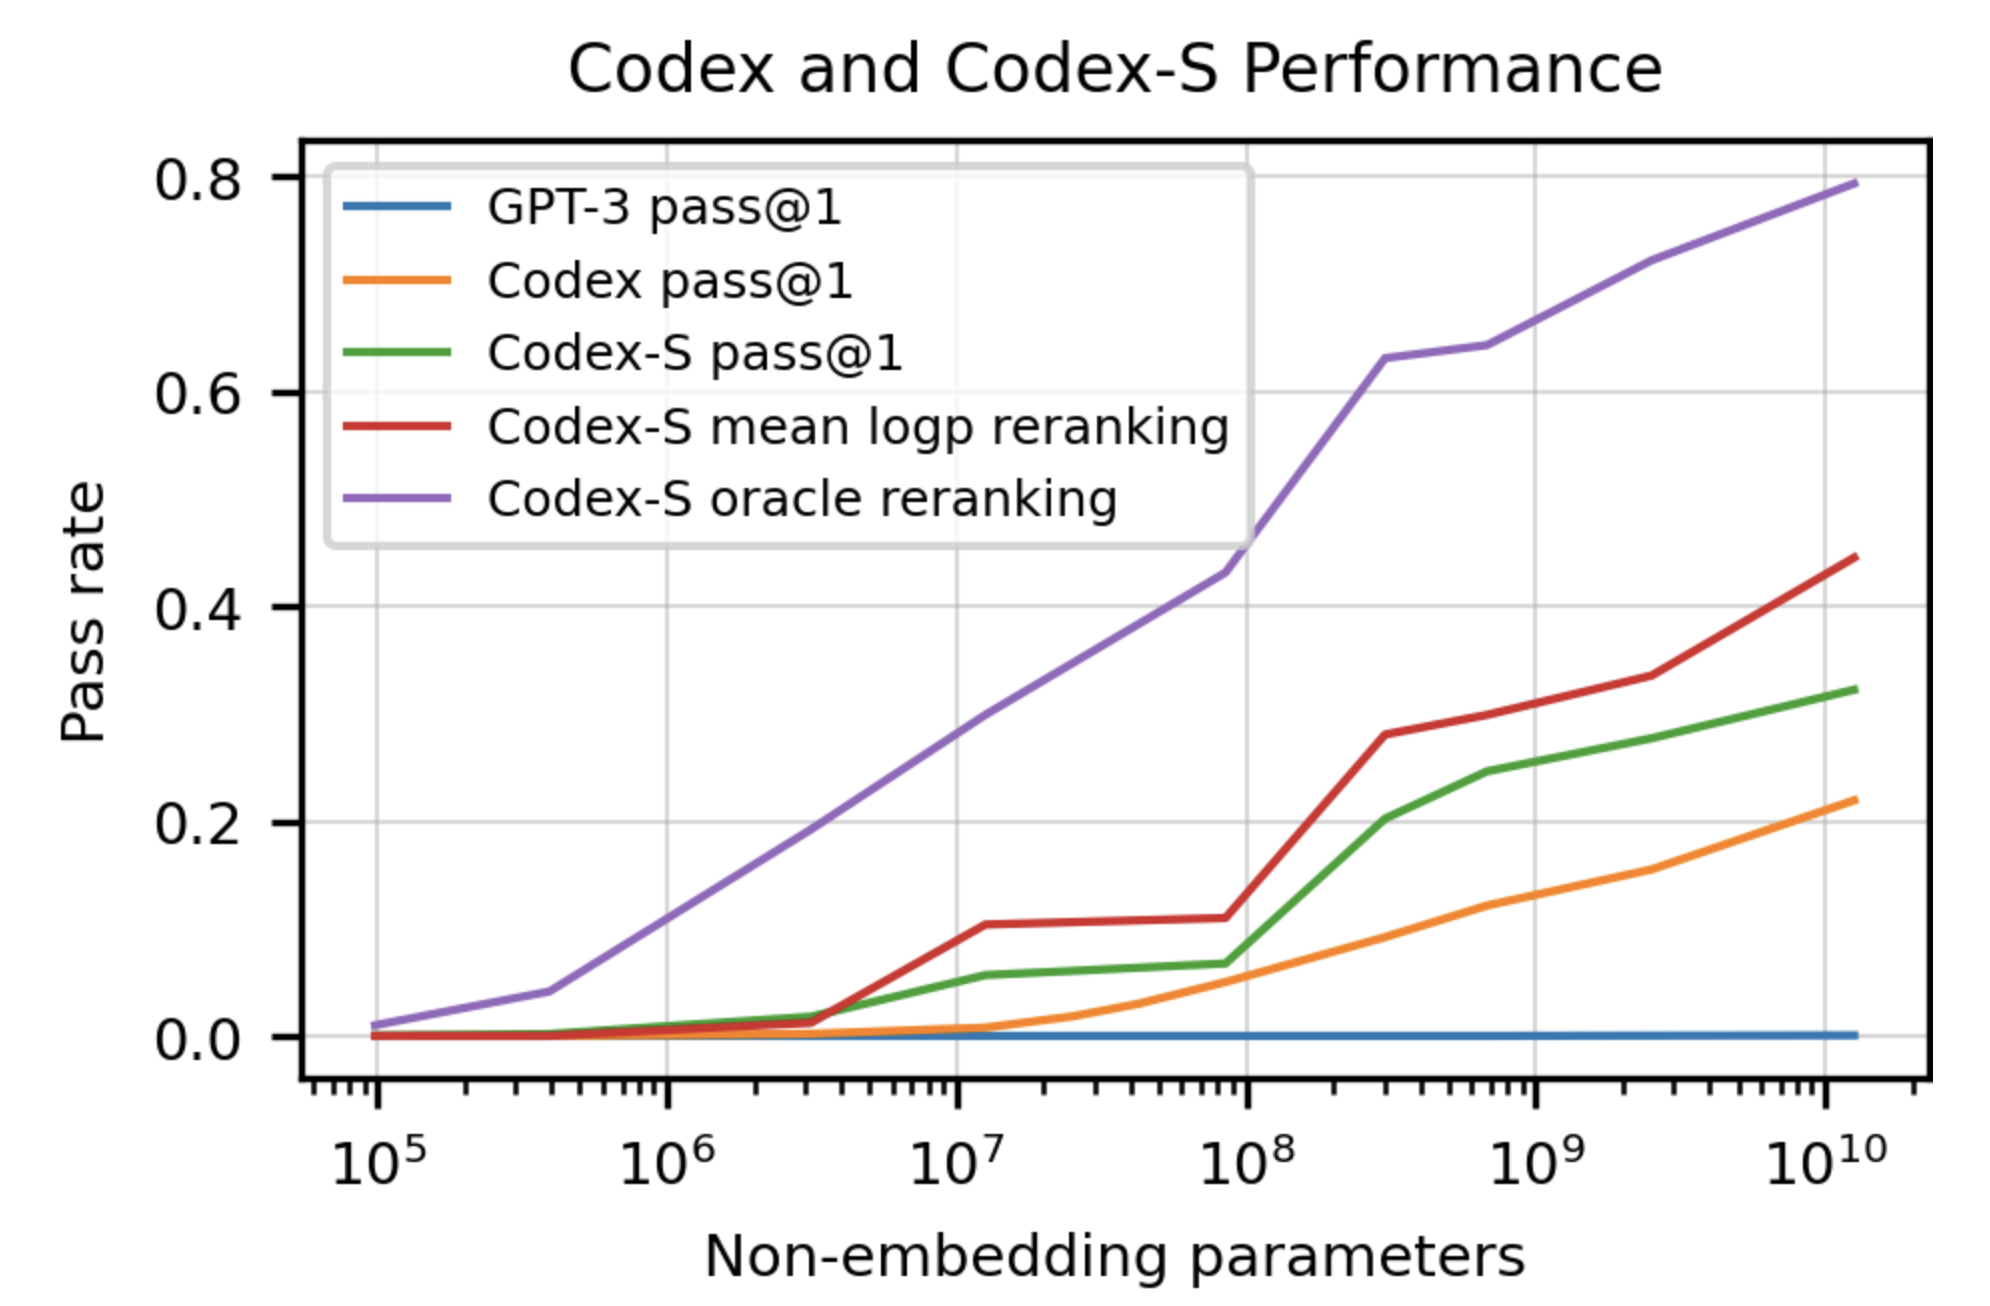
\includegraphics[width=0.6\textwidth]{s3.png}
\end{center}

\refline{\href{https://arxiv.org/abs/2107.03374}{M. Chen et al., ``Evaluating Large Language Models Trained on Code, arXiv (2021)}.}
\end{frame}

% 35
\begin{frame}[fragile]{Docstring complexity}
\tiny
\begin{columns}[T,totalwidth=\textwidth]
\column{0.49\textwidth}
\begin{block}{Composing building blocks}
The 13 building blocks are chained by concatenating:
\begin{itemize}
  \item their one-line descriptions into a docstring, and
  \item their one-line implementations into a code body.
\end{itemize}

\begin{lstlisting}
def string_manipulation(s: str):
    """
    This function takes a string as input, then
    returns the result of performing the following
    sequence of manipulations:
    - make every other character uppercase
    - replace spaces with triple spaces
    """
    s = "".join(char.upper() if i % 2 == 0 else char
                for i, char in enumerate(s))
    s = s.replace(" ", "   ")
    return s
\end{lstlisting}
\end{block}

\column{0.49\textwidth}
\begin{block}{Results}
    \begin{center} 
    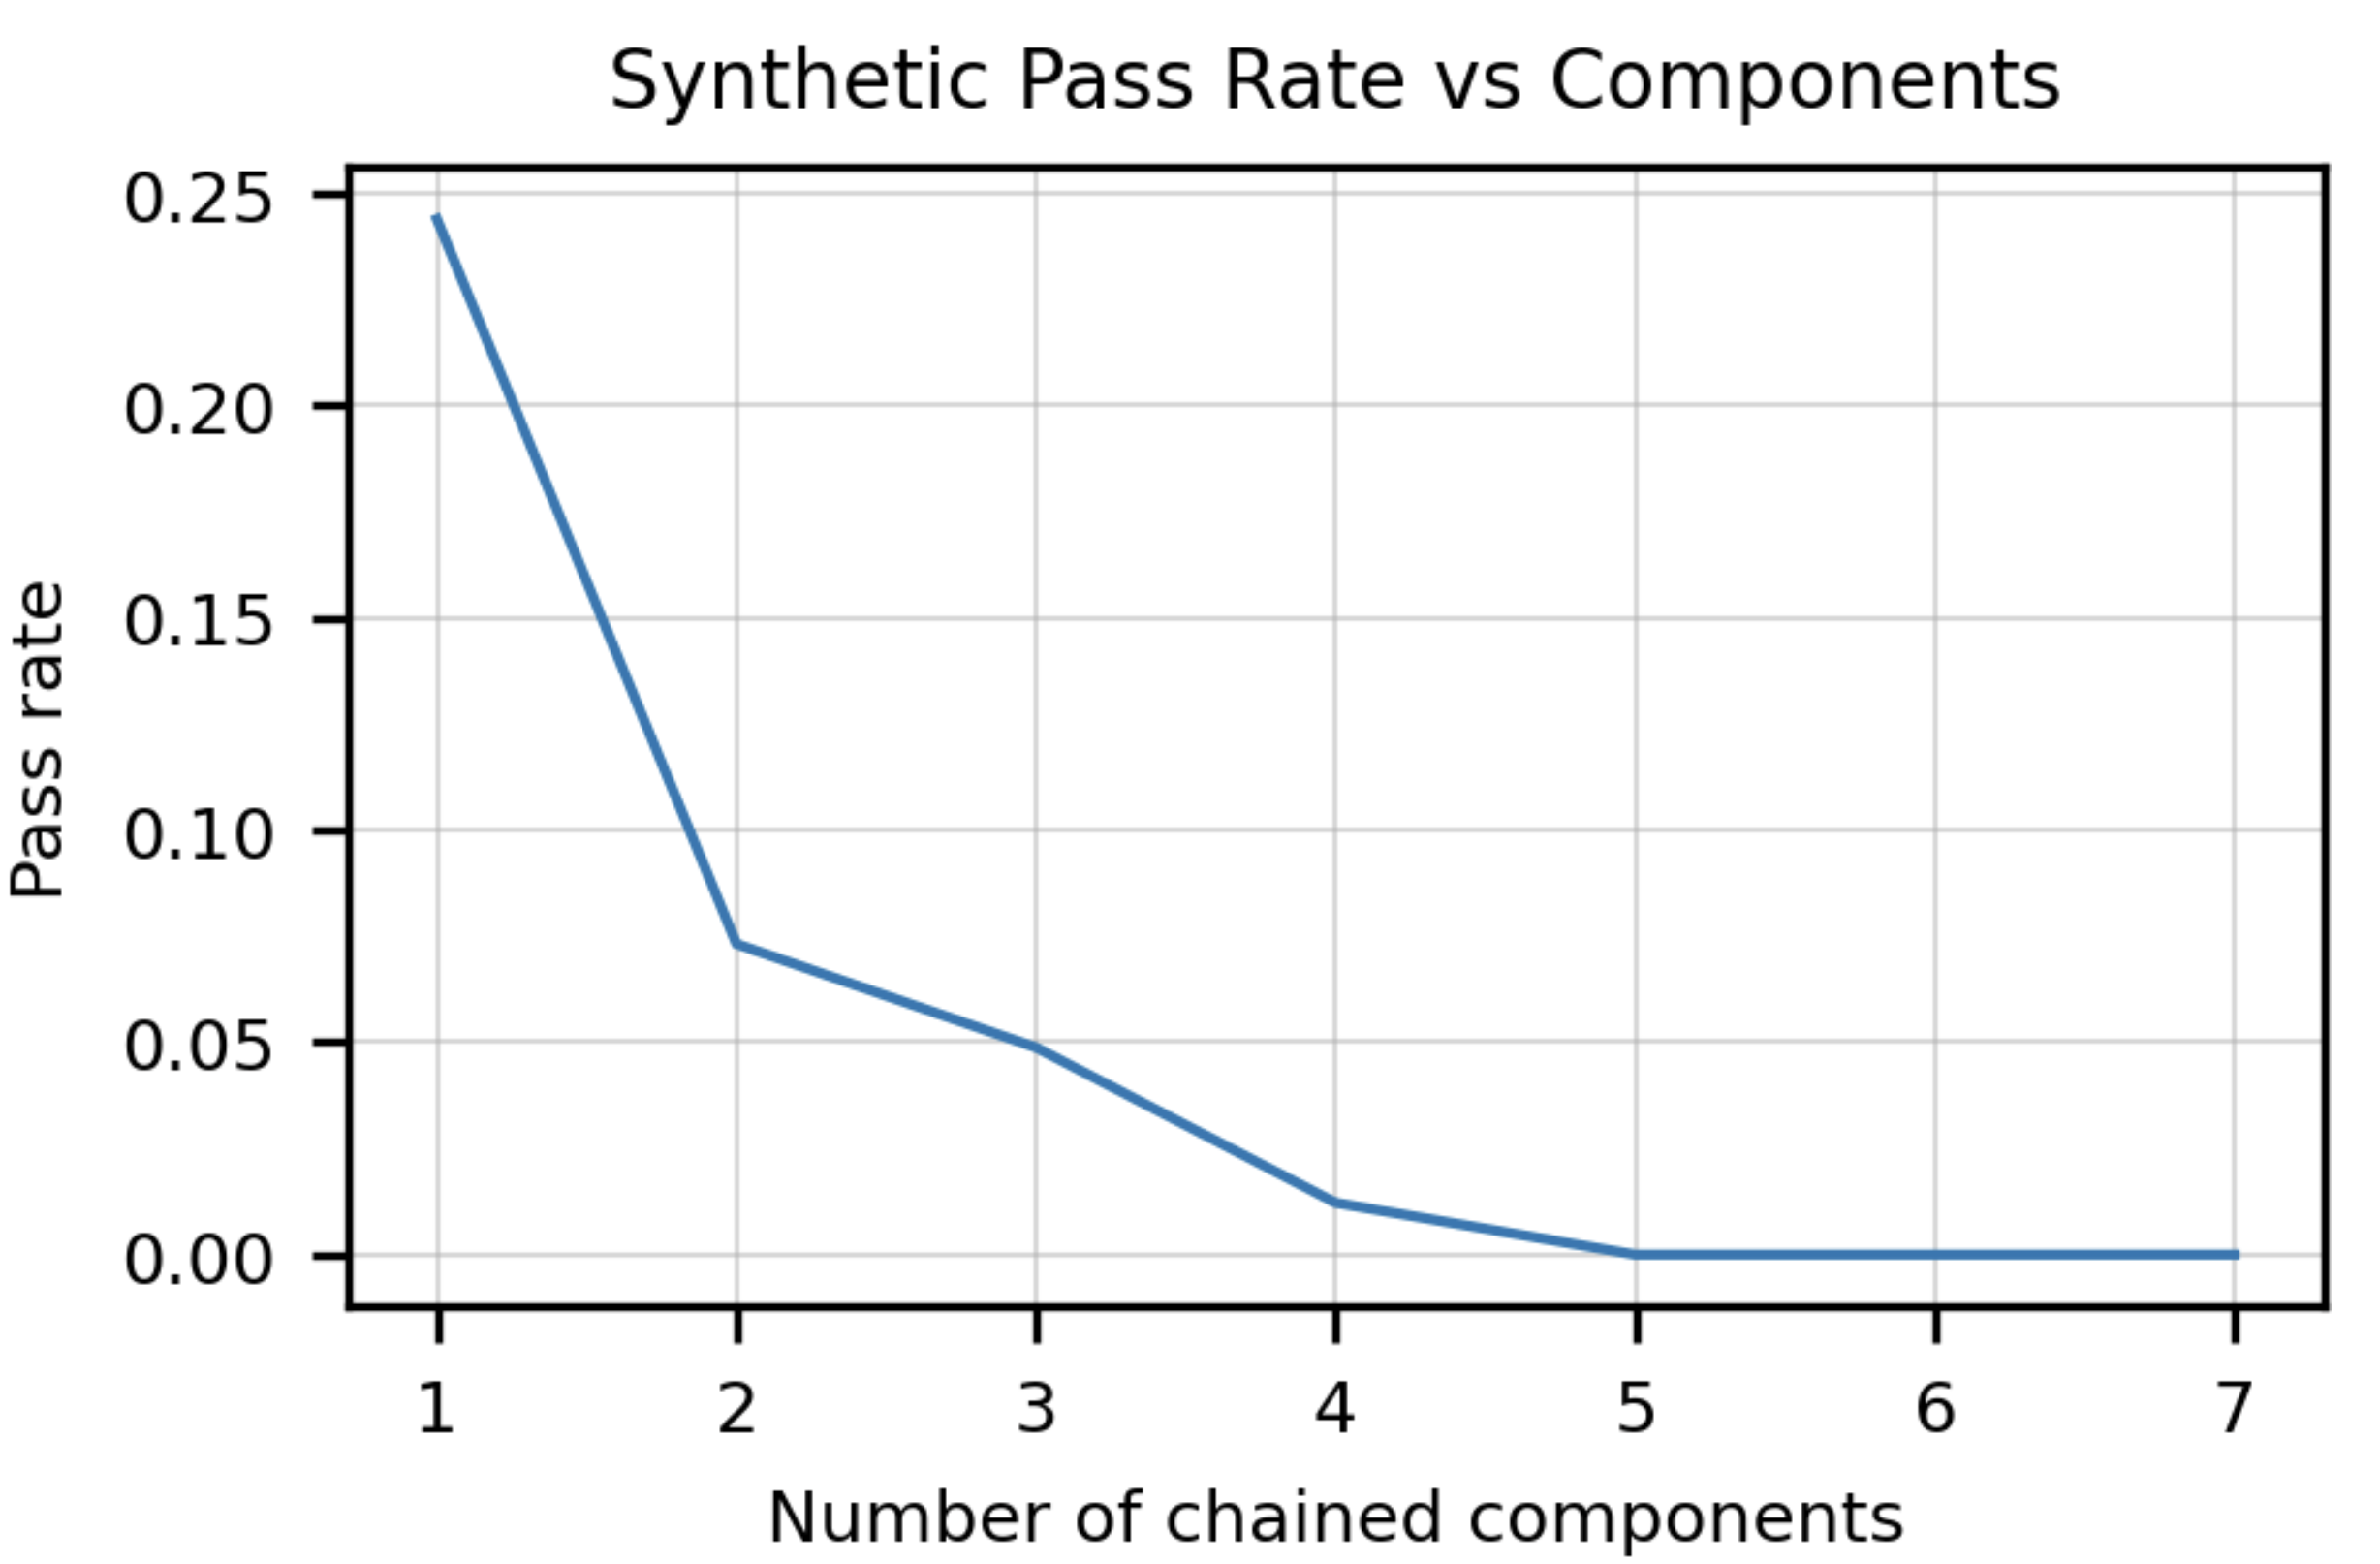
\includegraphics[width=0.6\textwidth]{docstr.png}
    \end{center}

\begin{itemize}
  \item As each component is added, the pass rate drops by about \textbf{2--3x}.
  \item Human programmers do not show the same degradation once they can chain two operations.
  \item Codex also makes variable-binding mistakes when many variables are mentioned.
\end{itemize}
\end{block}

\begin{alertblock}{Example binding failure}
Prompt idea: ``Add 3 to \texttt{y}, then subtract 4 from both \texttt{x} and \texttt{w}. Return the product of the four numbers.''

Observed failure: the generated code subtracts 4 from \texttt{x} but forgets to subtract 4 from \texttt{w}, and only multiplies two numbers.
\end{alertblock}
\end{columns}

\refline{\href{https://arxiv.org/abs/2107.03374}{M. Chen et al., ``Evaluating Large Language Models Trained on Code, arXiv (2021)}.}
\end{frame}

% limitations-summary
\begin{frame}{Limitations: where the method breaks}
\scriptsize
\begin{columns}[T,totalwidth=\textwidth]
\column{0.49\textwidth}
\begin{block}{Benchmark and evaluation limits}
\begin{itemize}
  \item \textbf{HumanEval is small and narrow}: only 164 problems, Python-only, and mostly single-function synthesis.
  \item \textbf{pass@k can look stronger than real one-shot use}: many-sample success is not the same as a reliable first answer.
  \item The benchmark omits repository context, debugging loops, retrieval, code review, and long-horizon maintenance.
\end{itemize}
\end{block}

\column{0.49\textwidth}
\begin{alertblock}{Model failure modes}
\begin{itemize}
  \item Performance degrades on longer and more compositional docstrings.
  \item Multi-function prompts and more realistic full-program settings are harder than HumanEval.
  \item Generated code can be plausible but still wrong, insecure, or misaligned with user intent.
\end{itemize}
\end{alertblock}

\begin{exampleblock}{Takeaway}
Codex is best viewed as a strong candidate generator plus verification story, not as a fully reliable end-to-end software engineer.
\end{exampleblock}
\end{columns}

\refline{\href{https://arxiv.org/abs/2107.03374}{M. Chen et al., ``Evaluating Large Language Models Trained on Code,'' arXiv (2021)}; \href{https://proceedings.neurips.cc/paper/2021/hash/c24cd76e1ce41366a4bbe8a49b02a028-Abstract.html}{D. Hendrycks et al., ``Measuring Coding Challenge Competence With APPS,'' NeurIPS (2021)}.}
\end{frame}


% 37
\begin{frame}{Broader Impacts and Hazard Analysis}
\scriptsize
\begin{columns}[T,totalwidth=\textwidth]
\column{0.49\textwidth}
\begin{block}{Applications of Codex}
\begin{itemize}
  \item onboarding users to new codebases,
  \item reducing context switches for experienced coders,
  \item enabling non-programmers to write specifications,
  \item producing draft implementations,
  \item aiding education and exploratory coding.
\end{itemize}
\end{block}

\column{0.49\textwidth}
\begin{block}{Hazard analysis and over-reliance}
\begin{itemize}
  \item Main risks: generated code may not match user intent, and the system may be misused.
  \item The analysis is framed in terms of risk factors rather than full product safety design.
  \item Over-reliance is a central concern, especially for novice programmers.
  \item Generated code may look correct but still be wrong or insecure.
  \item Automation bias makes this especially dangerous: people often trust automated suggestions too much.
  \item Human oversight remains necessary.
\end{itemize}
\end{block}
\end{columns}

\refline{\href{https://arxiv.org/abs/2107.03374}{M. Chen et al., ``Evaluating Large Language Models Trained on Code, arXiv (2021)}; \href{https://arxiv.org/abs/1904.02069}{N. Leveson, ``Improving the Standard Risk Matrix: Part 1, (2019)}.}
\end{frame}

% discussion
\begin{frame}{What happened after Codex?}
\scriptsize
\begin{block}{Three directions the line of work took next}
\begin{enumerate}
  \item \textbf{Harder generation and filtering}: systems such as AlphaCode pushed large-scale sampling and selection on competition-style tasks.
  \item \textbf{Open code LMs}: models such as StarCoder and Code Llama broadened access, reproducibility, and multilingual code modeling.
  \item \textbf{More realistic ML4SE evaluation}: benchmarks such as SWE-bench shifted attention from isolated functions toward repository-level issue resolution.
\end{enumerate}
\end{block}

% \begin{alertblock}{Connection to ML4SE more broadly}
% The field moved from code completion to \textbf{software engineering systems}: generation plus repository context, testing, reranking, tool use, and human oversight.
% \end{alertblock}
Codex did not solve software engineering. It changed the field by giving a compelling first demonstration, a reusable benchmark story, and a new default question for code LMs: not ``can it write code?'' but ``can it solve tasks we can execute and verify?''

% \begin{exampleblock}{Bottom line}
% \end{exampleblock}

\refline{\href{https://arxiv.org/abs/2203.07814}{Y. Li et al., ``Competition-Level Code Generation with AlphaCode,'' Science (2022)}; \href{https://arxiv.org/abs/2305.06161}{L. Ben Allal et al., ``StarCoder: May the Source Be with You!,'' arXiv (2023)}; \href{https://arxiv.org/abs/2308.12950}{B. Roziere et al., ``Code Llama: Open Foundation Models for Code,'' arXiv (2023)}; \href{https://arxiv.org/abs/2310.06770}{J. Jimenez et al., ``SWE-bench: Can Language Models Resolve Real-World GitHub Issues?,'' ICLR (2024)}.}
\end{frame}


% 53
\begin{frame}{Summary}
\small
\begin{block}{Summary}
\begin{itemize}
  \item The paper showed that a code-specialized language model can solve a non-trivial fraction of docstring-to-function tasks.
  \item Its deeper contribution was methodological: code generation should be judged by \textbf{functional correctness}, not just by textual similarity.
  \item The strongest results rely on sampling, reranking, and task-aligned fine-tuning, so benchmark success should not be confused with reliable one-shot software engineering.
  \item Historically, Codex helped launch the modern code-assistant era and influenced the move toward stronger benchmarks and more realistic ML4SE settings.
\end{itemize}
\end{block}

\refline{\href{https://arxiv.org/abs/2107.03374}{M. Chen et al., ``Evaluating Large Language Models Trained on Code, arXiv (2021)}.}
\end{frame}

\appendix
\begin{frame}[plain]
\centering
{\fontsize{26}{28}\selectfont\bfseries Q\&A\par}
\vfill
% \refline{\href{https://arxiv.org/abs/2107.03374}{M. Chen et al., ``Evaluating Large Language Models Trained on Code,'' arXiv (2021).}}
\end{frame}

% % 14
% \begin{frame}[fragile]{Prompting for evaluation}
% \scriptsize
% \begin{columns}[T,totalwidth=\textwidth]
% \column{0.52\textwidth}
% \begin{block}{Prompting to compute \texttt{pass@k}}
% Each HumanEval problem is assembled into a prompt made from the function signature, the docstring, and any examples.
% \begin{lstlisting}
% def incr_list(l: list):
%     """Return list with elements incremented by 1.
%     >>> incr_list([1, 2, 3])
%     [2, 3, 4]
%     >>> incr_list([5, 3, 5, 2, 3, 3, 9, 0, 123])
%     [6, 4, 6, 3, 4, 4, 10, 1, 124]
%     """
% \end{lstlisting}
% Sampling continues until one of the following stop tokens is encountered:
% \texttt{'\textbackslash nclass'}, \texttt{'\textbackslash ndef'}, \texttt{'\textbackslash n\#'}, \texttt{'\textbackslash nif'}, or \texttt{'\textbackslash nprint'}.
% \end{block}

% \column{0.44\textwidth}
% \begin{block}{Sampling details}
% \begin{itemize}
%   \item Nucleus sampling with \(p=0.95\) is used for all sampling evaluation.
%   \item For the simple single-function prompt on the slide, Codex 12B reaches about \textbf{pass@1 = 0.9}.
% \end{itemize}
% \end{block}

% \begin{alertblock}{Multi-function prompts}
% The paper notes a dramatic degradation when the prompt contains multiple functions. In the example on the slide, Codex 12B gets only about \textbf{pass@1 = 0.005}.
% \end{alertblock}
% \end{columns}

% \refline{\href{https://arxiv.org/abs/2107.03374}{M. Chen et al., ``Evaluating Large Language Models Trained on Code, arXiv (2021)}; \href{https://arxiv.org/abs/1904.09751}{A. Holtzman et al., ``The Curious Case of Neural Text Degeneration, ICLR (2020)}.}
% \end{frame}

% % 16
% \begin{frame}{Loss scaling and temperature}
% \scriptsize
% \begin{columns}[T,totalwidth=\textwidth]
% \column{0.49\textwidth}
% \begin{block}{Loss scaling}
% \begin{itemize}
%   \item Language model losses often follow a power law.
%   \item The paper finds a similar pattern for Codex test loss on a held-out GitHub validation set.
% \end{itemize}
% \end{block}

% \begin{center}
%     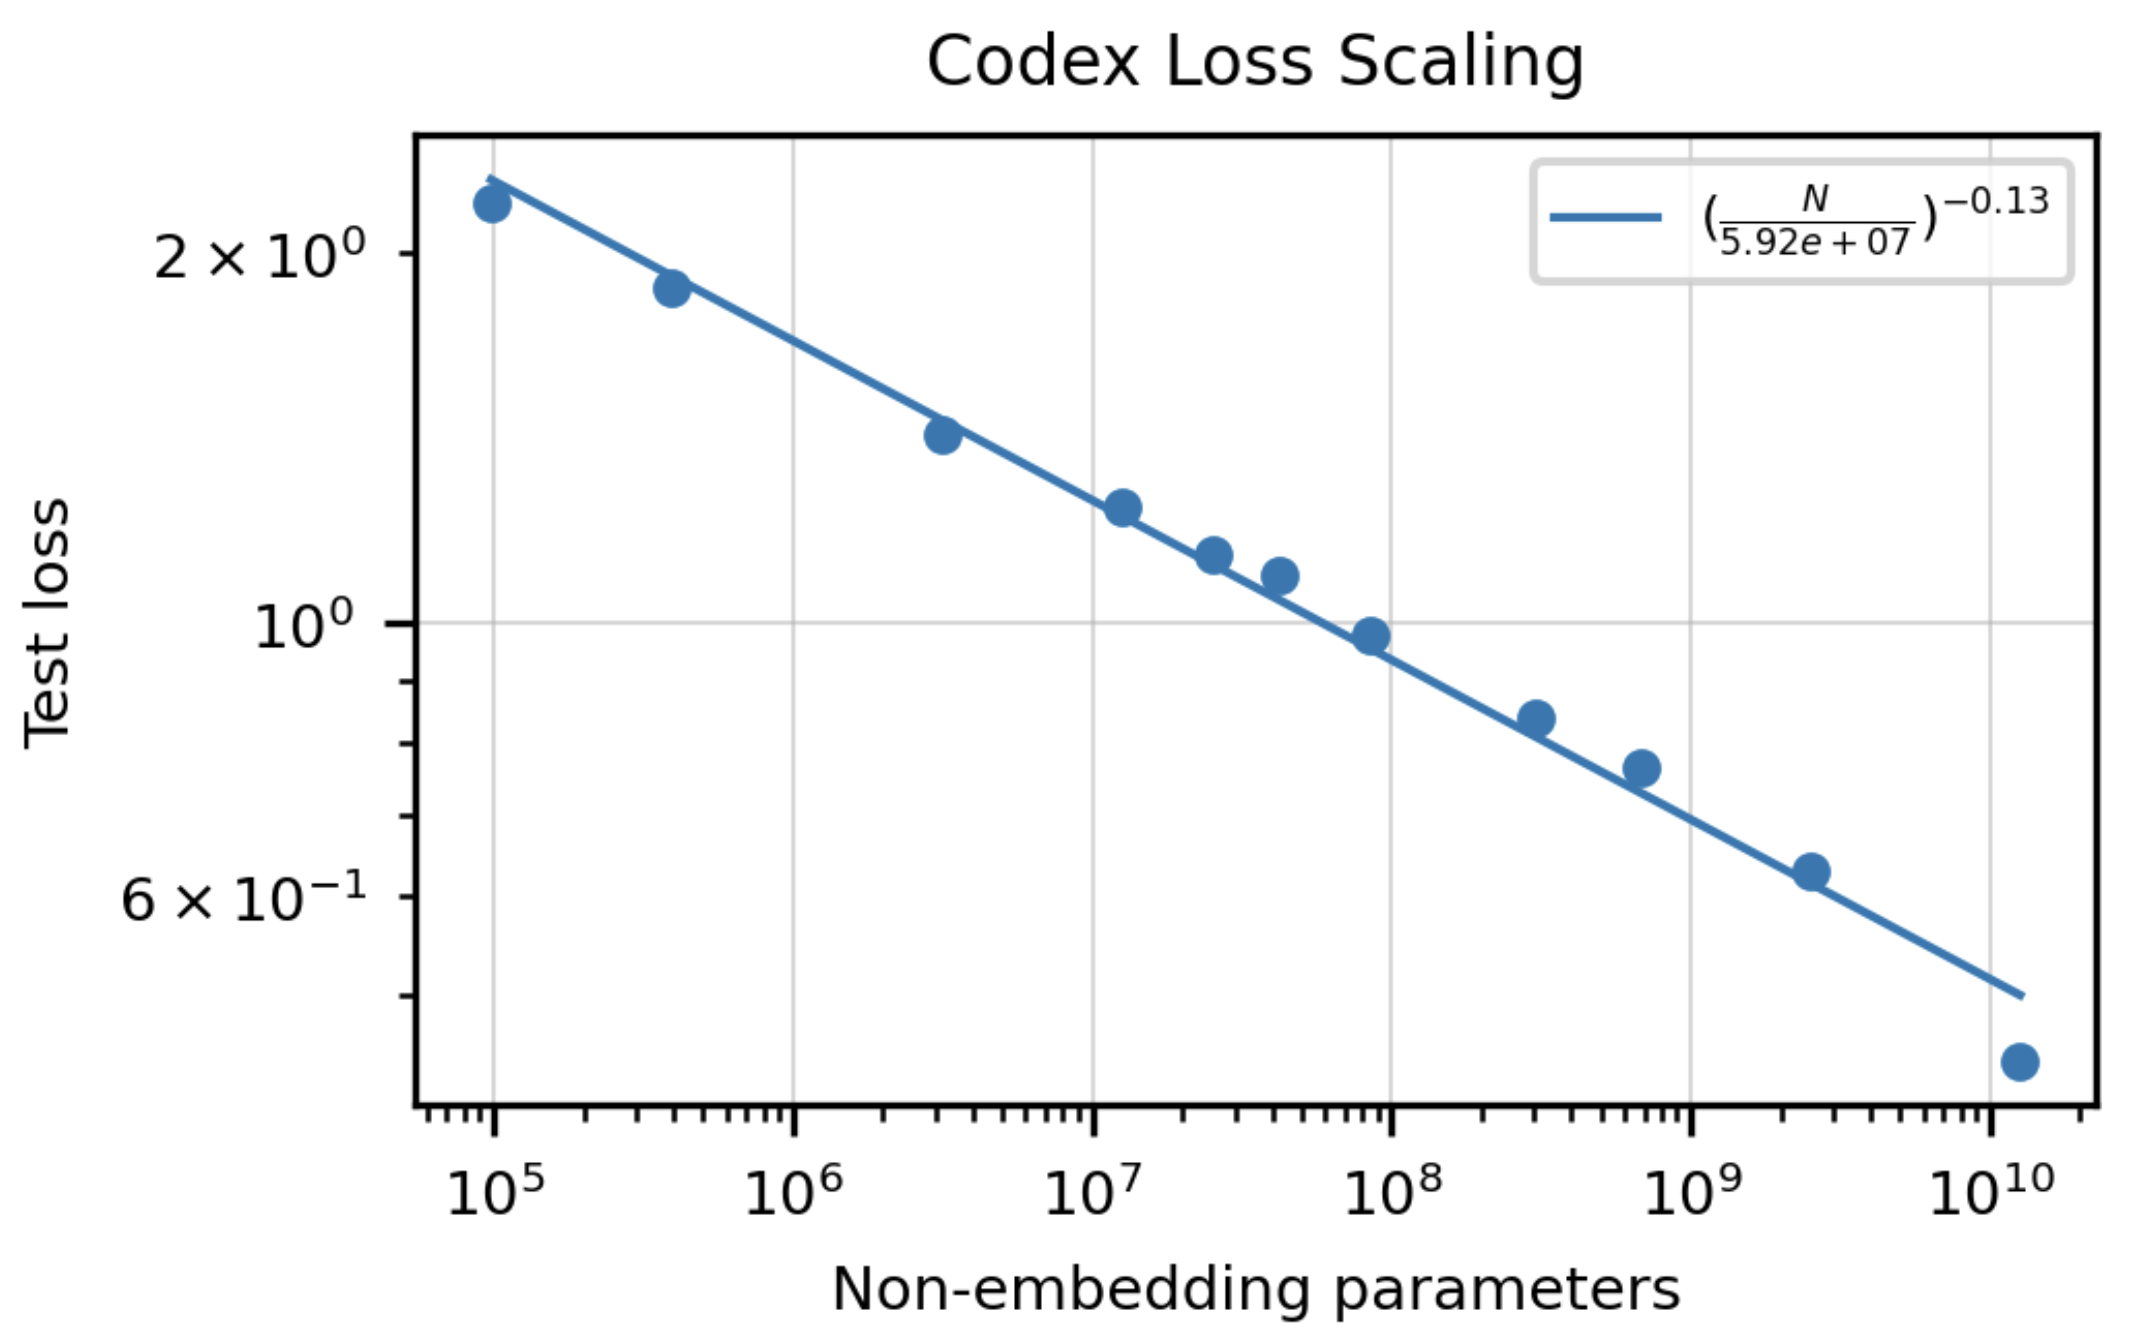
\includegraphics[width=0.9\textwidth]{loss1.png}
% \end{center}
% \column{0.49\textwidth}
% \begin{block}{Sampling temperature}
% % \begin{itemize}
% %   \item Best temperature depends on \(k\).
% %   \item For larger \(k\), higher temperatures work better because \texttt{pass@k} rewards whether the model generates \emph{any} correct solution.
% % \end{itemize}
% \end{block}

% \begin{center}
%     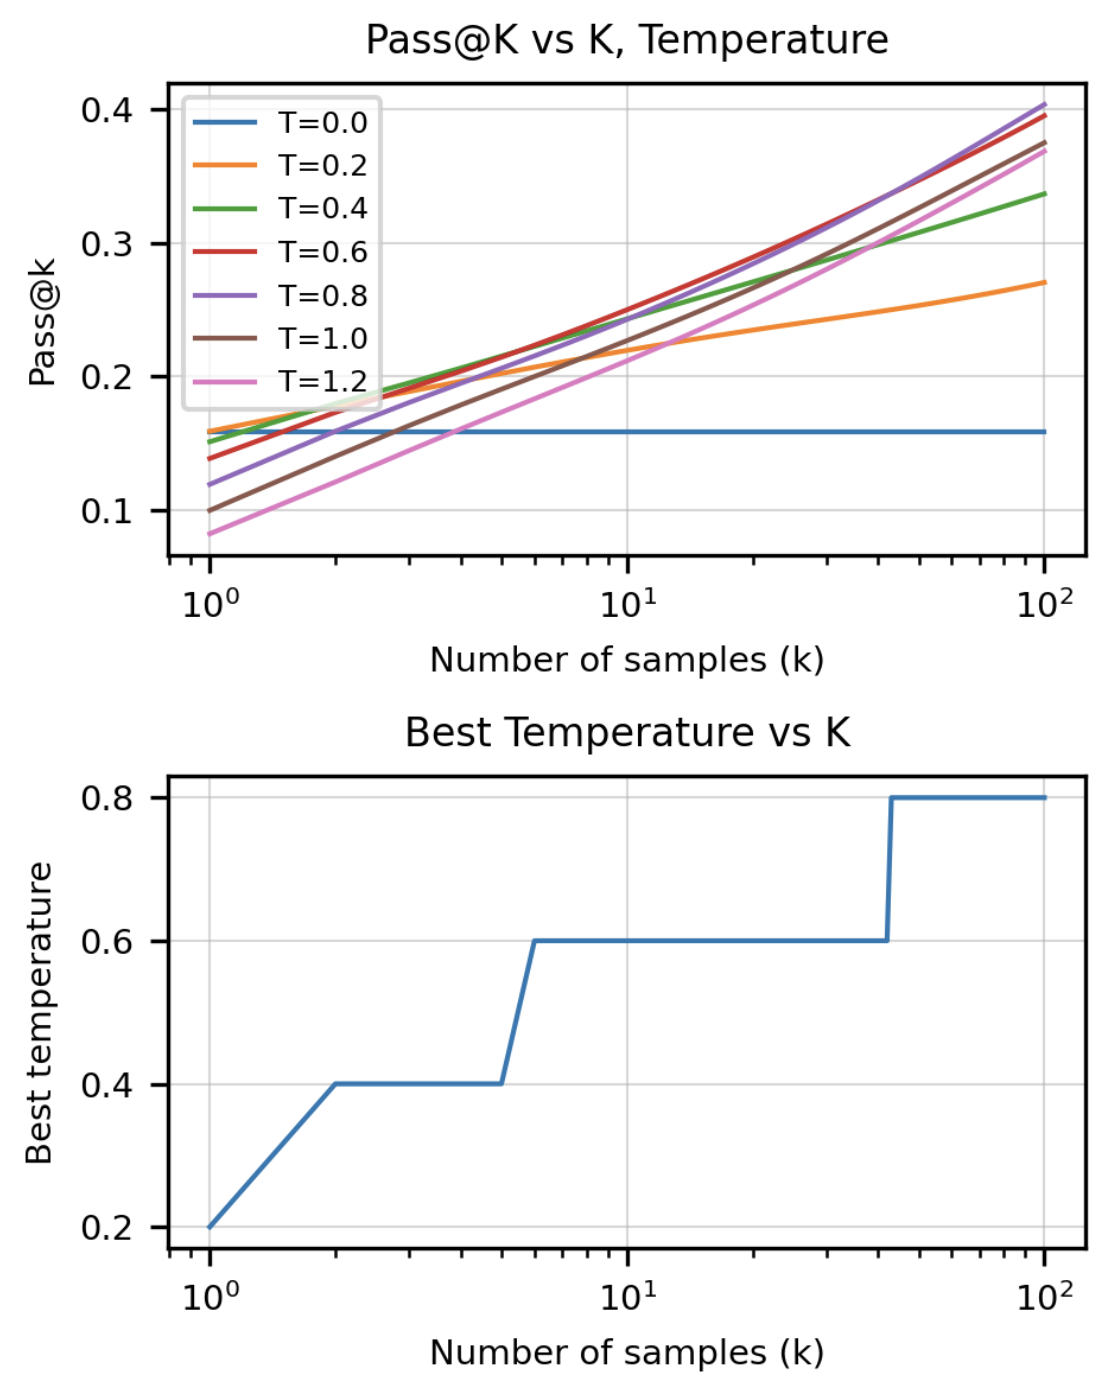
\includegraphics[width=0.9\textwidth]{loss2.png}
% \end{center}
% \end{columns}

% \refline{\href{https://arxiv.org/abs/2001.08361}{J. Kaplan et al., ``Scaling Laws for Neural Language Models, arXiv (2020)}; \href{https://arxiv.org/abs/2107.03374}{M. Chen et al., ``Evaluating Large Language Models Trained on Code, arXiv (2021)}.}
% \end{frame}

% % 17
% \begin{frame}{Model scaling at optimal temperatures}
% \small
% \begin{block}{Model scaling}
% For a \textbf{679M}-parameter model, the best temperatures are:
% \begin{itemize}
%   \item \(T^* = 0.2\) for \texttt{pass@1}
%   \item \(T^* = 0.8\) for \texttt{pass@100}
% \end{itemize}
% \end{block}

% \begin{center}
%     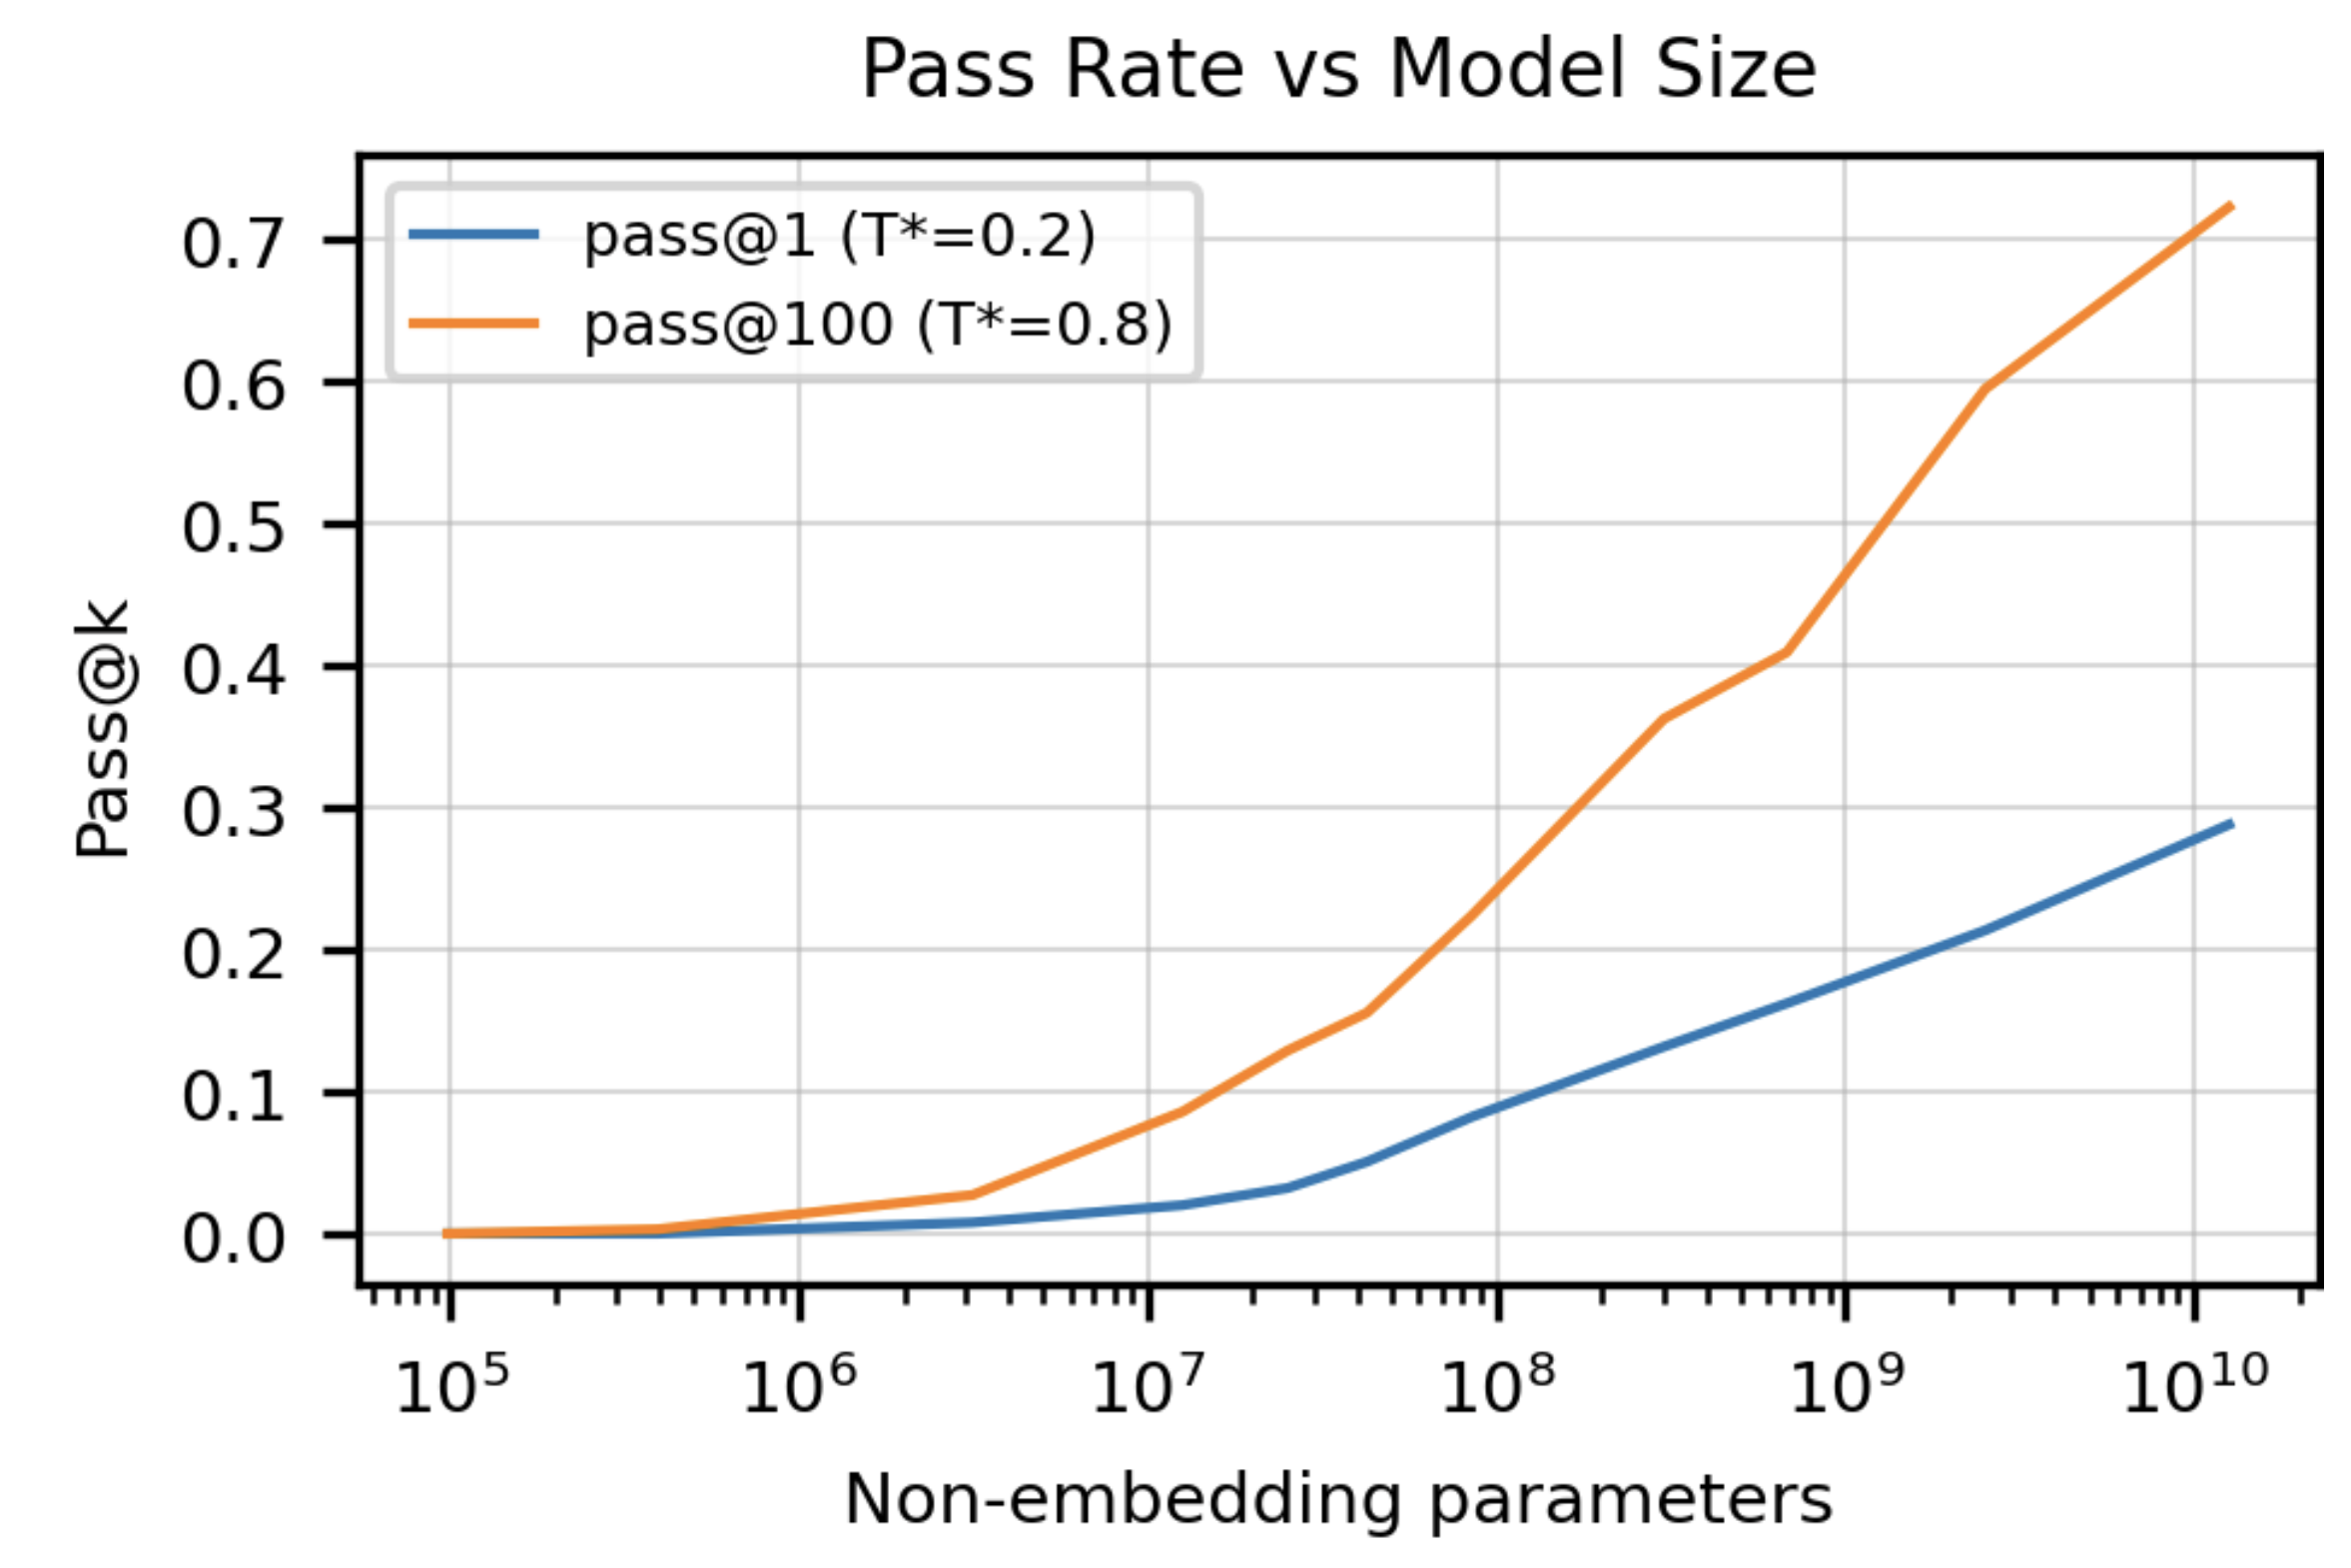
\includegraphics[width=0.7\textwidth]{temp0.png}
% \end{center}
% \refline{\href{https://arxiv.org/abs/2107.03374}{M. Chen et al., ``Evaluating Large Language Models Trained on Code, arXiv (2021)}.}
% \end{frame}

% % 18
% \begin{frame}{Sampling heuristics and BLEU score}
% \scriptsize
% \begin{columns}[T,totalwidth=\textwidth]
% \column{0.49\textwidth}
% \begin{block}{Effectiveness of sampling heuristics}
% \begin{itemize}
%   \item \texttt{pass@k} can be interpreted as evaluating the best out of \(k\) samples.
%   \item An oracle that knows the unit tests is the upper bound.
%   \item Without an oracle, a practical goal is to select one sample among \(k\) candidates.
%   \item For Codex 12B at \(T=0.8\), the best non-oracle heuristic is \textbf{mean log-probability}.
% \end{itemize}
% \end{block}

% \begin{center}
%     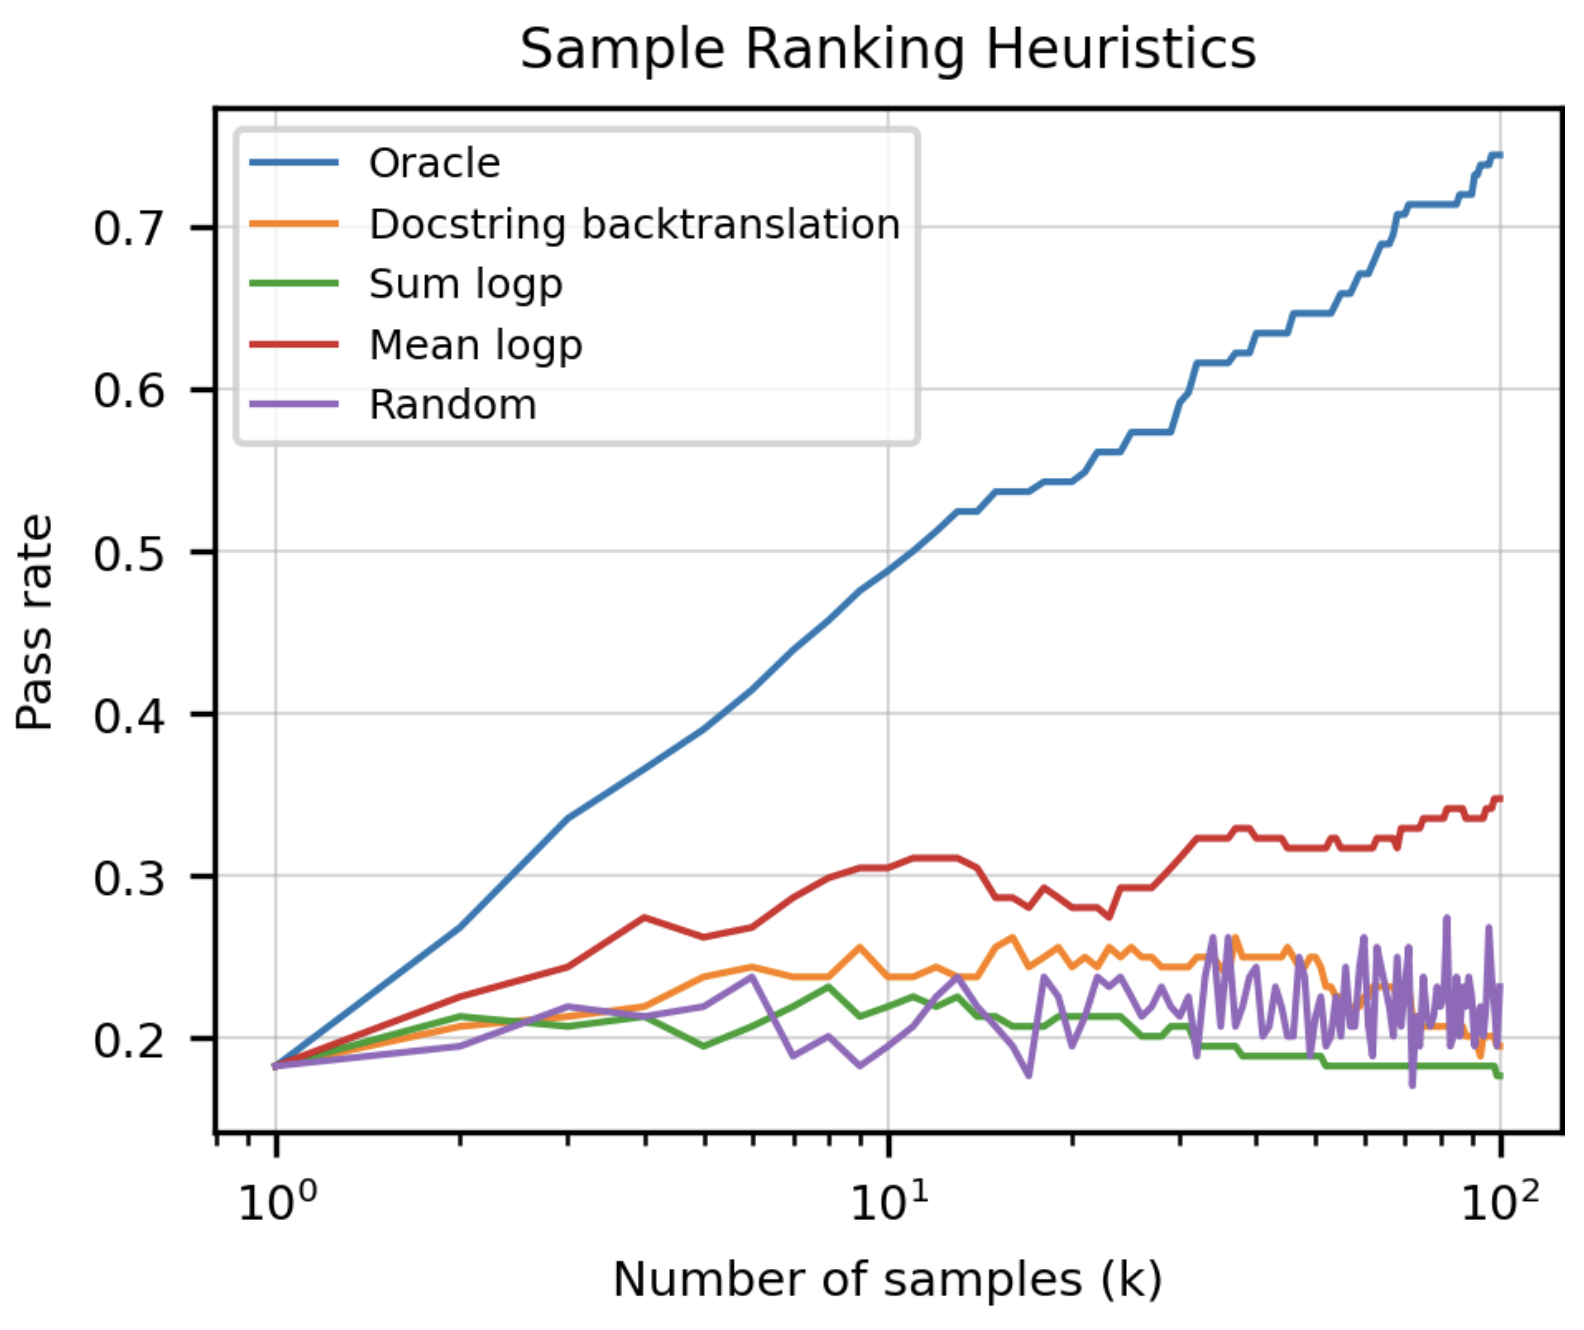
\includegraphics[width=0.9\textwidth]{bleu1.png}
% \end{center}
% \column{0.49\textwidth}
% \begin{block}{BLEU score correlation}
% \begin{itemize}
%   \item BLEU scores are computed for HumanEval Codex 12B samples at \(T=0.8\).
%   \item The comparison is made against reference solutions.
%   \item Correct and wrong solutions are \textbf{not cleanly separable} by BLEU.
% \end{itemize}
% \end{block}

% \begin{center}
%     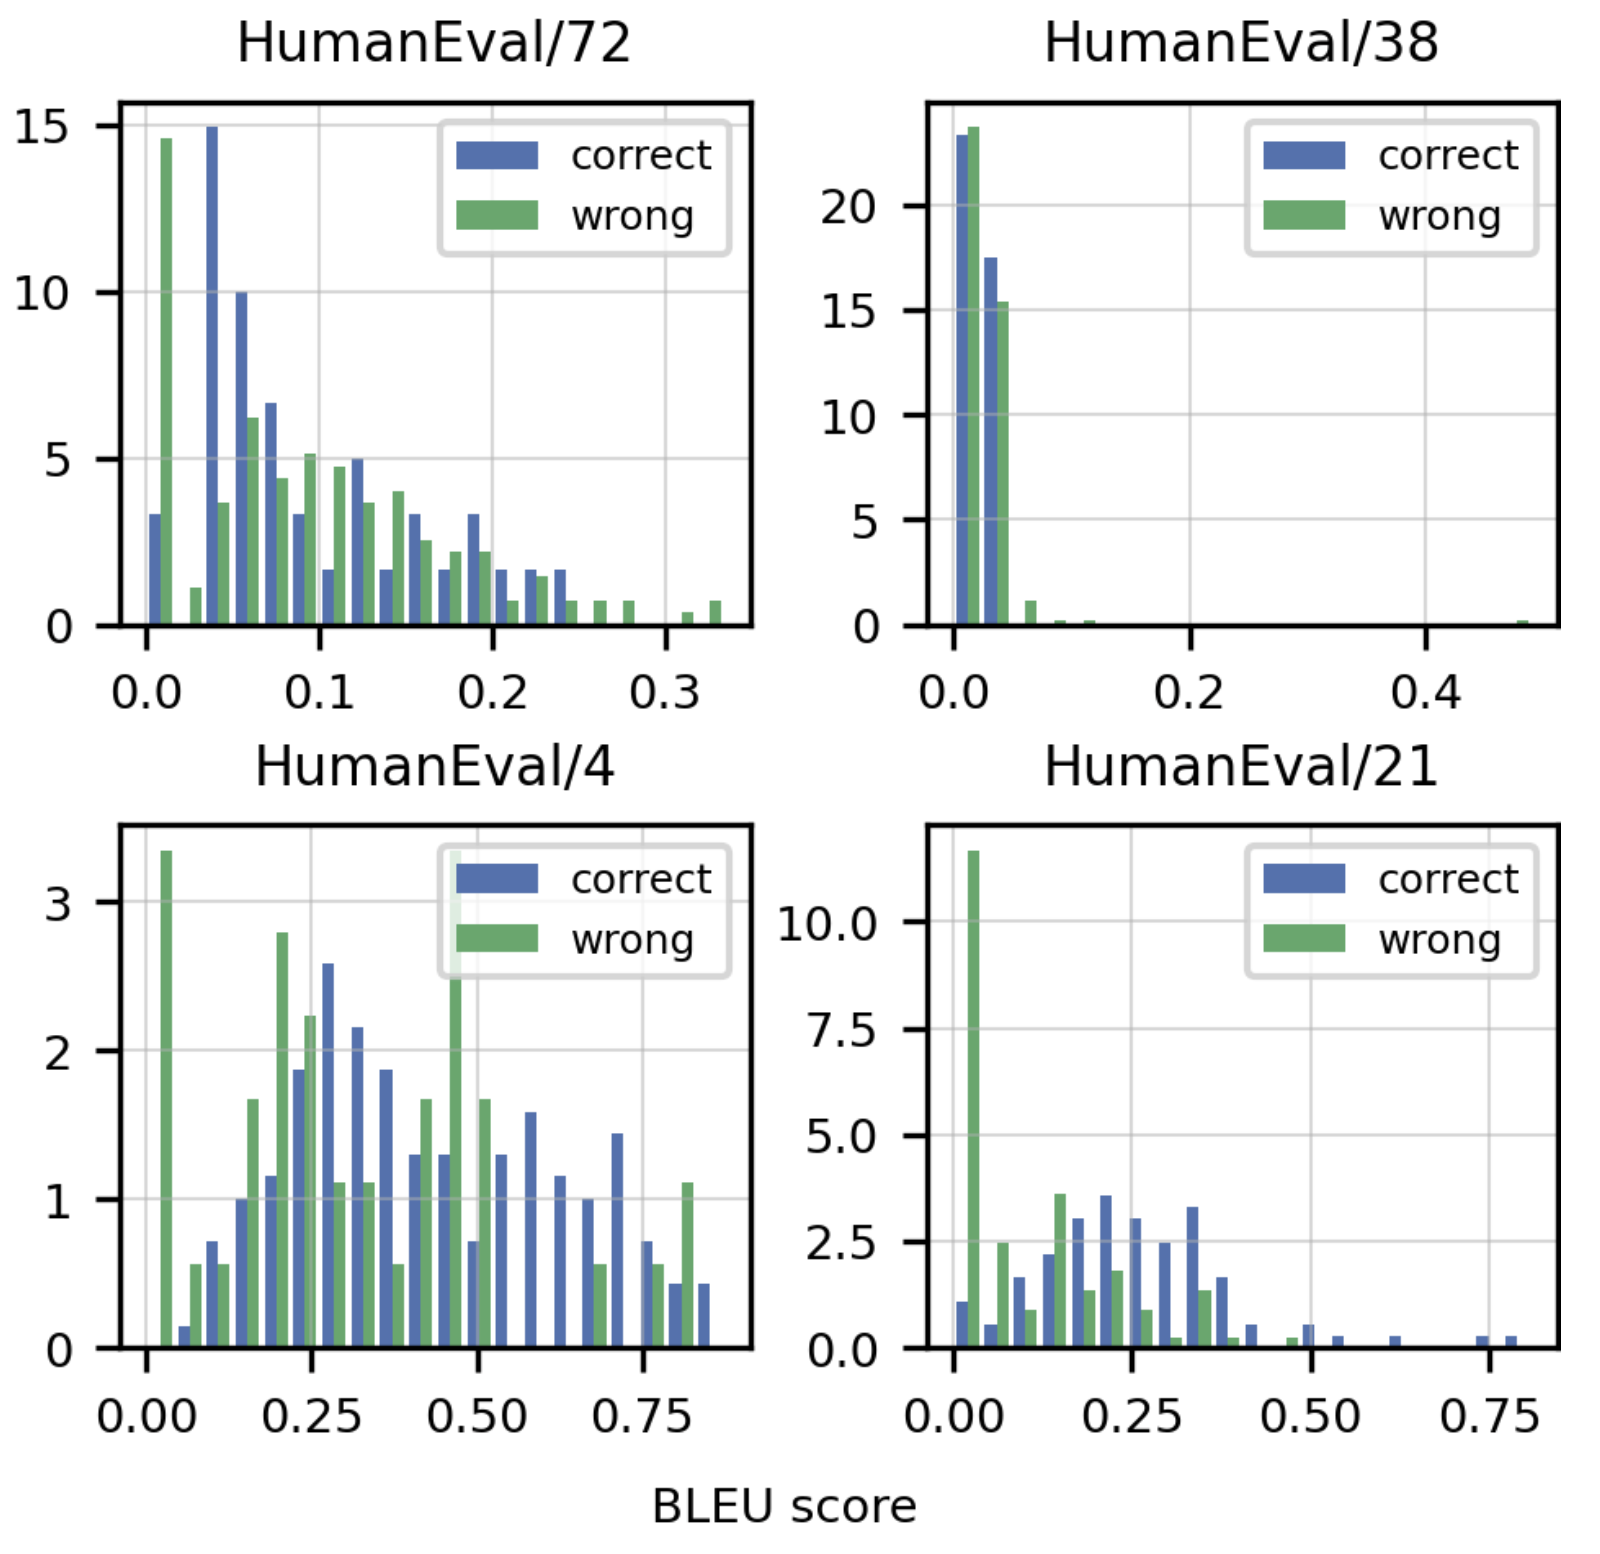
\includegraphics[width=0.9\textwidth]{bleu2.png}
% \end{center}
% \end{columns}

% \refline{\href{https://arxiv.org/abs/2107.03374}{M. Chen et al., ``Evaluating Large Language Models Trained on Code, arXiv (2021)}.}
% \end{frame}

% % 21
% \begin{frame}[fragile]{Code generation examples}
% \tiny
% \begin{block}{Prompt}
% \begin{lstlisting}
% def is_prime(n):
%     """Return true if a given number is prime.
%     >>> is_prime(6)
%     False
%     >>> is_prime(101)
%     True
%     >>> is_prime(4)
%     False
%     >>> is_prime(1)
%     False
%     """
% \end{lstlisting}
% 8 random samples are shown on the original slide (temperature 0.8).
% \end{block}

% \begin{columns}[T,totalwidth=\textwidth]
% \column{0.49\textwidth}
% \begin{block}{Completions 1--3 (wrong)}
% \begin{itemize}
%   \item \textbf{Completion 1:}
% \begin{lstlisting}
% for i in range(2, n):
%     if n % i == 0:
%         return False
% return True
% \end{lstlisting}
% Fails for \(n=1\) because it returns True.
%   \item \textbf{Completion 2:} exactly the same as Completion 1.
%   \item \textbf{Completion 3:}
% \begin{lstlisting}
% # TODO: implement this function
% pass
% \end{lstlisting}
% Fails all unit tests.
% \end{itemize}
% \end{block}

% \column{0.49\textwidth}
% \begin{block}{Completions 4--5}
% \begin{itemize}
%   \item \textbf{Completion 4 (correct):}
%     handles \(n<2\), handles 2, rejects evens, and tests odd divisors up to \(\sqrt n\).
%   \item \textbf{Completion 5 (wrong):}
%     uses a helper to test divisibility up to \(\sqrt n\), but still returns True for \(n=1\).
% \end{itemize}

% \end{block}
% \end{columns}

% \refline{\href{https://arxiv.org/abs/2107.03374}{M. Chen et al., ``Evaluating Large Language Models Trained on Code, arXiv (2021)}.}
% \end{frame}

% % 22
% \begin{frame}[fragile]{Code generation examples}
% \tiny
% \begin{columns}[T,totalwidth=\textwidth]
% \column{0.49\textwidth}
% \begin{block}{Completions 6--8}
% \begin{itemize}
%   \item \textbf{Completion 6 (correct):}
% \begin{lstlisting}
% prime = True
% if n == 1:
%     return False
% for i in range(2, n):
%     if n % i == 0:
%         prime = False
% return prime
% \end{lstlisting}
% Exhaustive check, but correct.
%   \item \textbf{Completion 7 (wrong):} repeats the same bug as Completion 1.
%   \item \textbf{Completion 8 (correct):} efficient primality test based on checking divisibility by 2, 3, and then numbers of the form \(6k\pm 1\).
% \end{itemize}
% \end{block}

% \column{0.49\textwidth}
% \begin{block}{Why \(6k \pm 1\) matters}
% For primes greater than 3, any candidate factor must be of the form \(6k \pm 1\).
% \begin{itemize}
%   \item Numbers of the form \(6k\), \(6k+2\), and \(6k+4\) are divisible by 2.
%   \item Numbers of the form \(6k+3\) are divisible by 3.
%   \item So after handling 2 and 3, only \(6k-1\) and \(6k+1\) remain worth testing.
% \end{itemize}
% This makes Completion 8 faster than checking every number up to \(n\).
% \end{block}
% \end{columns}

% \refline{\href{https://arxiv.org/abs/2107.03374}{M. Chen et al., ``Evaluating Large Language Models Trained on Code, arXiv (2021)}; \href{https://en.wikipedia.org/wiki/Primality_test}{Wikipedia, ``Primality test, accessed for the standard 6k±1 observation}}
% \end{frame}

% % 8
% \begin{frame}{Nuances of pass@k estimation}
%     \scriptsize
%     \begin{columns}[T,totalwidth=\textwidth]
%     \column{0.53\textwidth}
%     \begin{block}{Estimating \texttt{pass@k}}
%     Aim: estimate the probability that among \(k\) samples, at least one is correct.
%     \begin{itemize}
%       \item If the true probability of a correct sample is \(p\), then:
%       \[
%       \Pr(\text{none correct}) = (1-p)^k,
%       \qquad
%       \mathrm{pass@}k = 1 - (1-p)^k.
%       \]
%       \item A naive plug-in estimate \(1-(1-\hat p)^k\) from \(\hat p = \mathrm{pass@}1\) systematically underestimates performance.
%       \item It also makes results look better simply by drawing more samples from the same pool.
%       \item The paper's estimator instead compares tasks across different numbers of samples in a consistent way.
%     \end{itemize}
%     \end{block}
    
%     \column{0.43\textwidth}
%     \begin{block}{Comparing estimators for pass@k}
%         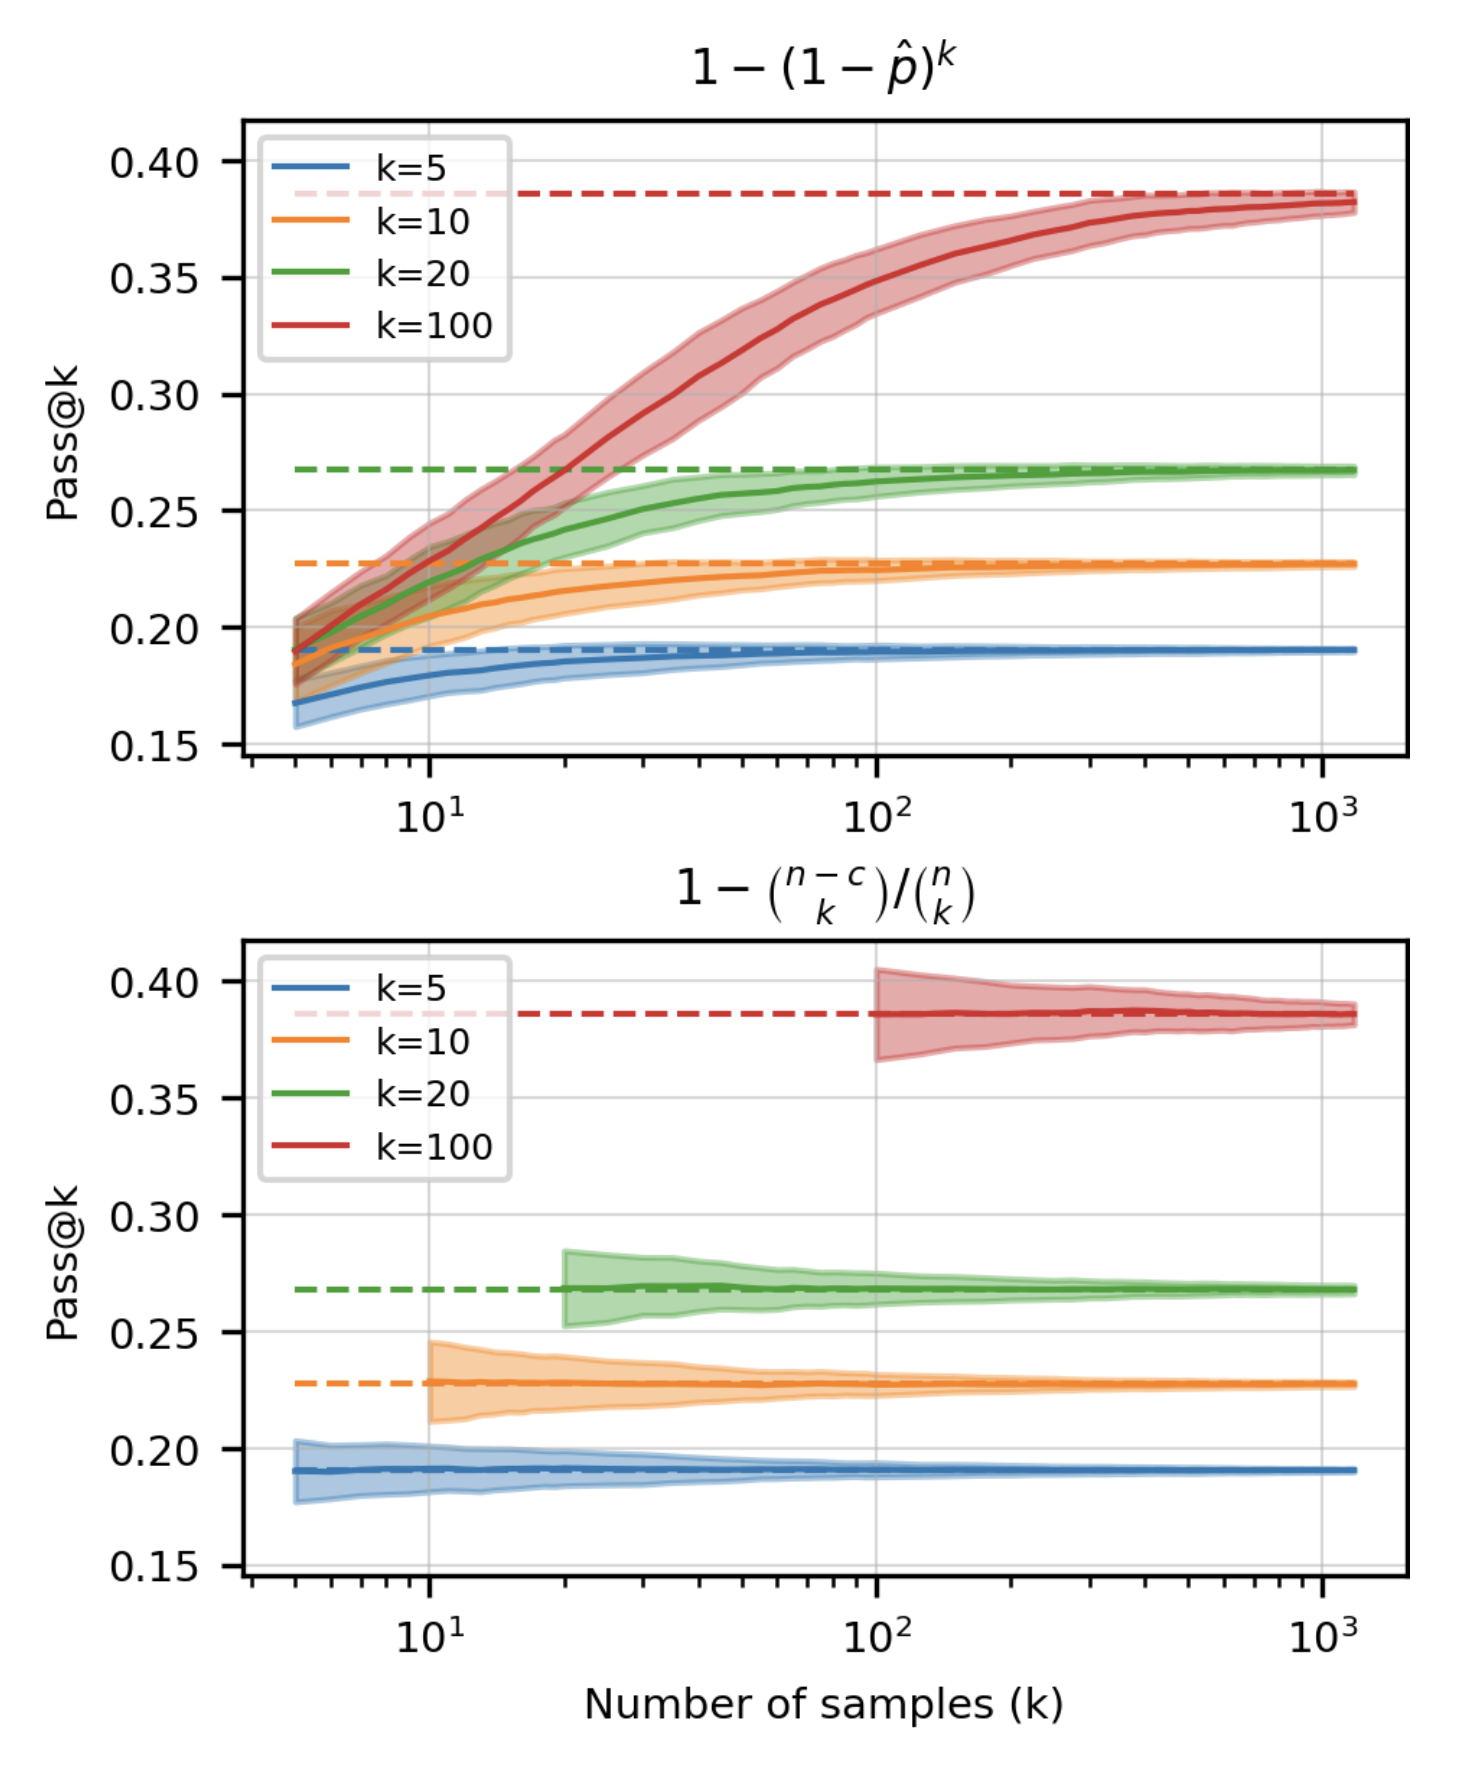
\includegraphics[width=0.78\textwidth]{estim.png}\end{block}
    
%     % \begin{alertblock}{Key point}
%     % Slightly higher initial variance is acceptable because the estimator enables fairer comparisons across different sample budgets.
%     % \end{alertblock}
%     \end{columns}
    
%     \refline{\href{https://arxiv.org/abs/2107.03374}{M. Chen et al., ``Evaluating Large Language Models Trained on Code, arXiv (2021)}.}
%     \end{frame}
    
%     % 9
%     \begin{frame}{Nuances of pass@k estimation}
%     \scriptsize
%     \begin{block}{Why the proposed estimator is unbiased}
%     The second term in
%     \[
%     \mathbb{E}\left[1 - \frac{\binom{n-c}{k}}{\binom{n}{k}}\right]
%     \]
%     directly estimates the probability of drawing \textbf{only failed samples} when choosing \(k\) items without replacement from \(n\) candidates.
%     \end{block}
    
%     \begin{columns}[T,totalwidth=\textwidth]
%     \column{0.48\textwidth}
%     \begin{block}{Setup}
%     \begin{itemize}
%       \item Let \(c \sim \mathrm{Binom}(n,p)\), where \(p\) is \(\mathrm{pass@}1\).
%       \item If \(n-c < k\), then \(\binom{n-c}{k}=0\), so the estimator returns 1.
%       \item Otherwise, the estimator computes the probability that all \(k\) chosen samples are failures.
%     \end{itemize}
%     \end{block}
    
%     \column{0.48\textwidth}
%     \begin{block}{Sketch of the derivation}
%     \[
%     \mathbb{E}\!\left[\frac{\binom{n-c}{k}}{\binom{n}{k}}\right]
%     = \sum_{i=0}^{n-k} \frac{\binom{n-i}{k}}{\binom{n}{k}}\binom{n}{i}p^i(1-p)^{n-i}
%     \]
%     \[
%     = (1-p)^k \sum_{i=0}^{n-k} \binom{n-k}{i}p^i(1-p)^{n-k-i}
%     = (1-p)^k
%     \]
%     Therefore,
%     \[
%     \mathbb{E}[\mathrm{estimator}] = 1-(1-p)^k = \mathrm{pass@}k.
%     \]
%     \end{block}
%     \end{columns}
    
%     \refline{\href{https://arxiv.org/abs/2107.03374}{M. Chen et al., ``Evaluating Large Language Models Trained on Code, arXiv (2021)}.}
%     \end{frame}
    
%     % 10
%     \begin{frame}[fragile]{Implementing the pass@k estimator}
%     \scriptsize
%     \begin{columns}[T,totalwidth=\textwidth]
%     \column{0.47\textwidth}
%     \begin{block}{Numerically stable implementation}
%     \begin{lstlisting}
%     def pass_at_k(n, c, k):
%         """
%         n: total number of samples
%         c: number of correct samples
%         k: k in pass@k
%         """
%         if n - c < k:
%             return 1.0
%         return 1.0 - np.prod(
%             1.0 - k / np.arange(n - c + 1, n + 1)
%         )
%     \end{lstlisting}
%     \end{block}
    
%     \column{0.49\textwidth}
%     \begin{block}{Rationale for \(n-c < k\)}
%     If fewer than \(k\) failed samples exist, then it is impossible to draw \(k\) failures without replacement:
%     \[
%     \binom{n-c}{k}=0
%     \quad\Rightarrow\quad
%     1 - \frac{\binom{n-c}{k}}{\binom{n}{k}} = 1.
%     \]
%     \end{block}
    
%     \begin{exampleblock}{Rationale for \(n-c \ge k\)}
%     Rewrite the combinatorial ratio as a stable product:
%     \[
%     \frac{\binom{n-c}{k}}{\binom{n}{k}}
%     = \prod_{j=n-c+1}^{n}\left(1-\frac{k}{j}\right)
%     \]
%     which is exactly what the NumPy implementation computes.
%     \end{exampleblock}
%     \end{columns}
    
%     \refline{\href{https://arxiv.org/abs/2107.03374}{M. Chen et al., ``Evaluating Large Language Models Trained on Code, arXiv (2021)}.}
%     \end{frame}


\end{document}

\end{document}
